% Options for packages loaded elsewhere
\PassOptionsToPackage{unicode}{hyperref}
\PassOptionsToPackage{hyphens}{url}
%
\documentclass[
]{article}
\usepackage{amsmath,amssymb}
\usepackage{iftex}
\ifPDFTeX
  \usepackage[T1]{fontenc}
  \usepackage[utf8]{inputenc}
  \usepackage{textcomp} % provide euro and other symbols
\else % if luatex or xetex
  \usepackage{unicode-math} % this also loads fontspec
  \defaultfontfeatures{Scale=MatchLowercase}
  \defaultfontfeatures[\rmfamily]{Ligatures=TeX,Scale=1}
\fi
\usepackage{lmodern}
\ifPDFTeX\else
  % xetex/luatex font selection
\fi
% Use upquote if available, for straight quotes in verbatim environments
\IfFileExists{upquote.sty}{\usepackage{upquote}}{}
\IfFileExists{microtype.sty}{% use microtype if available
  \usepackage[]{microtype}
  \UseMicrotypeSet[protrusion]{basicmath} % disable protrusion for tt fonts
}{}
\makeatletter
\@ifundefined{KOMAClassName}{% if non-KOMA class
  \IfFileExists{parskip.sty}{%
    \usepackage{parskip}
  }{% else
    \setlength{\parindent}{0pt}
    \setlength{\parskip}{6pt plus 2pt minus 1pt}}
}{% if KOMA class
  \KOMAoptions{parskip=half}}
\makeatother
\usepackage{xcolor}
\usepackage[margin=1in]{geometry}
\usepackage{graphicx}
\makeatletter
\def\maxwidth{\ifdim\Gin@nat@width>\linewidth\linewidth\else\Gin@nat@width\fi}
\def\maxheight{\ifdim\Gin@nat@height>\textheight\textheight\else\Gin@nat@height\fi}
\makeatother
% Scale images if necessary, so that they will not overflow the page
% margins by default, and it is still possible to overwrite the defaults
% using explicit options in \includegraphics[width, height, ...]{}
\setkeys{Gin}{width=\maxwidth,height=\maxheight,keepaspectratio}
% Set default figure placement to htbp
\makeatletter
\def\fps@figure{htbp}
\makeatother
\setlength{\emergencystretch}{3em} % prevent overfull lines
\providecommand{\tightlist}{%
  \setlength{\itemsep}{0pt}\setlength{\parskip}{0pt}}
\setcounter{secnumdepth}{-\maxdimen} % remove section numbering
\usepackage{float}
\usepackage{caption}
\usepackage{titlesec}
\usepackage{longtable}
\usepackage{booktabs}
\newcommand{\beginsection}{\clearpage}
\renewcommand{\thefigure}{S\arabic{figure}}
\renewcommand{\thetable}{S\arabic{table}}
\titleformat{\section}{\normalfont\Large\bfseries}{\thesection}{1em}{}[\vspace{-0.5\baselineskip}]
\usepackage{longtable}
\usepackage{booktabs}
\usepackage{array}
\usepackage{multirow}
\usepackage{wrapfig}
\usepackage{float}
\usepackage{colortbl}
\usepackage{pdflscape}
\usepackage{tabu}
\usepackage{threeparttable}
\usepackage{threeparttablex}
\usepackage[normalem]{ulem}
\usepackage{makecell}
\usepackage{xcolor}
\ifLuaTeX
  \usepackage{selnolig}  % disable illegal ligatures
\fi
\IfFileExists{bookmark.sty}{\usepackage{bookmark}}{\usepackage{hyperref}}
\IfFileExists{xurl.sty}{\usepackage{xurl}}{} % add URL line breaks if available
\urlstyle{same}
\hypersetup{
  pdftitle={Supplementary Material},
  hidelinks,
  pdfcreator={LaTeX via pandoc}}

\title{Supplementary Material}
\author{}
\date{\vspace{-2.5em}}

\begin{document}
\maketitle

This file contains supplementary tables and figures associated to the
paper
\emph{On the variation of structural divergence among residues in enzyme evolution},
by J. Echave and M. Carpentier.

\clearpage

\hypertarget{dataset}{%
\section{Dataset}\label{dataset}}

\nopagebreak

\begin{table}[!h]
\centering
\caption{\label{tab:unnamed-chunk-1}Dataset entries and reference protein}
\centering
\resizebox{\ifdim\width>\linewidth\linewidth\else\width\fi}{!}{
\fontsize{8}{10}\selectfont
\begin{tabular}[t]{rl>{\raggedright\arraybackslash}p{4cm}>{\raggedright\arraybackslash}p{4cm}>{\raggedright\arraybackslash}p{4cm}}
\toprule
M-CSA & PDB & Name & Source & Family\\
\midrule
2 & 1btl\_A & Beta-lactamase TEM & Escherichia coli & Class-A beta-lactamase family\\
15 & 1znb\_A & Metallo-beta-lactamase type 2 & Bacteroides fragilis & Metallo-beta-lactamase superfamily\\
71 & 1eug\_A & Uracil-DNA glycosylase & Escherichia coli B & Uracil-DNA glycosylase (UDG) superfamily\\
98 & 1bsz\_C & Peptide deformylase & Escherichia coli K-12 & Polypeptide deformylase family\\
109 & 1d3g\_A & Dihydroorotate dehydrogenase (quinone), mitochondrial & Homo sapiens & Dihydroorotate dehydrogenase family\\
148 & 1onr\_A & Name not found & Escherichia coli & Transaldolase family\\
151 & 1q0n\_A & 2-amino-4-hydroxy-6-hydroxymethyldihydropteridine pyrophosphokinase & Escherichia coli & HPPK family\\
160 & 1ako\_A & Exodeoxyribonuclease III & Escherichia coli K-12 & DNA repair enzymes AP/ExoA family\\
164 & 1ruv\_A & Ribonuclease pancreatic & Bos taurus & Pancreatic ribonuclease family\\
174 & 9pap\_A & Papain & Carica papaya & Peptidase C1 family\\
216 & 1ca2\_A & Carbonic anhydrase 2 & Homo sapiens & Alpha-carbonic anhydrase family\\
252 & 1igs\_A & Indole-3-glycerol phosphate synthase & Saccharolobus solfataricus & TrpC family\\
257 & 1xx2\_A & Beta-lactamase & Enterobacter cloacae & Class-C beta-lactamase family\\
258 & 1sml\_A & Metallo-beta-lactamase L1 type 3 & Stenotrophomonas maltophilia & Metallo-beta-lactamase superfamily\\
290 & 1zio\_A & Adenylate kinase & Geobacillus stearothermophilus & Adenylate kinase family\\
328 & 1lbm\_A & N-(5\&apos & Thermotoga maritima & TrpF family\\
351 & 1snz\_A & Galactose mutarotase & Homo sapiens & Aldose epimerase family\\
362 & 1d6o\_A & Peptidyl-prolyl cis-trans isomerase FKBP1A & Homo sapiens & FKBP-type PPIase family\\
376 & 1a4l\_A & Adenosine deaminase & Mus musculus & Metallo-dependent hydrolases superfamily\\
394 & 1aj0\_A & Dihydropteroate synthase & Escherichia coli & DHPS family\\
444 & 1cel\_A & Exoglucanase 1 & Trichoderma reesei & Glycosyl hydrolase 7 (cellulase C) family\\
462 & 1pnt\_A & Low molecular weight phosphotyrosine protein phosphatase & Bos taurus & Low molecular weight phosphotyrosine protein phosphatase family\\
467 & 1cv2\_A & Haloalkane dehalogenase & Sphingomonas paucimobilis & Haloalkane dehalogenase family\\
480 & 1czf\_A & Endopolygalacturonase II & Aspergillus niger & Glycosyl hydrolase 28 family\\
597 & 1uch\_A & Ubiquitin carboxyl-terminal hydrolase isozyme L3 & Homo sapiens & Peptidase C12 family\\
681 & 1gq8\_A & Pectinesterase & Daucus carota & Pectinesterase family\\
693 & 2rnf\_A & Ribonuclease 4 & Homo sapiens & Pancreatic ribonuclease family\\
749 & 1nml\_A & No information found & Marinobacter nauticus & No information found\\
814 & 1glo\_A & Cathepsin S & Homo sapiens & Peptidase C1 family\\
858 & 1mrq\_A & Aldo-keto reductase family 1 member C1 & Homo sapiens & Aldo/keto reductase family\\
877 & 1pbg\_A & 6-phospho-beta-galactosidase & Lactococcus lactis & Glycosyl hydrolase 1 family\\
908 & 1rtu\_A & Ribonuclease U2 & Ustilago sphaerogena & Ribonuclease U2 family\\
923 & 2acy\_A & Acylphosphatase-1 & Bos taurus & Acylphosphatase family\\
931 & 2pth\_A & Peptidyl-tRNA hydrolase & Escherichia coli K-12 & PTH family\\
\bottomrule
\end{tabular}}
\end{table}

\clearpage
\begin{table}
\centering
\caption{\label{tab:unnamed-chunk-2}Dataset properties}
\centering
\resizebox{\ifdim\width>\linewidth\linewidth\else\width\fi}{!}{
\fontsize{8}{10}\selectfont
\begin{threeparttable}
\begin{tabular}[t]{rrrrrrrll}
\toprule
M-CSA & N & <Id\%> & <RMSD> & Length & AS size & AS RMSD & CATH & EC\\
\midrule
2 & 6 & 43 & 1.04 & 263 & 6 & 1.78 & alpha/beta & Hydrolases\\
15 & 6 & 35 & 1.16 & 225 & 8 & 1.84 & alpha/beta & Hydrolases\\
71 & 8 & 43 & 1.08 & 223 & 4 & 1.49 & alpha/beta & Hydrolases\\
98 & 10 & 37 & 2.15 & 168 & 7 & 1.44 & alpha/beta & Hydrolases\\
109 & 4 & 44 & 1.31 & 359 & 7 & 2.65 & alpha/beta & Oxidoreductases\\
\addlinespace
148 & 5 & 53 & 1.06 & 316 & 5 & 2.09 & alpha/beta & Transferases\\
151 & 4 & 47 & 1.14 & 158 & 4 & 2.07 & alpha/beta & Transferases\\
160 & 10 & 34 & 1.49 & 256 & 7 & 2.63 & alpha/beta & Hydrolases\\
164 & 5 & 48 & 1.09 & 123 & 5 & 1.92 & alpha/beta & Lyases\\
174 & 12 & 43 & 1.01 & 212 & 4 & 1.57 & alpha/beta & Hydrolases\\
\addlinespace
216 & 5 & 39 & 1.09 & 256 & 6 & 2.27 & alpha/beta & Lyases\\
252 & 6 & 35 & 1.75 & 245 & 7 & 2.93 & alpha/beta & Lyases\\
257 & 10 & 45 & 0.94 & 359 & 6 & 1.48 & alpha/beta & Hydrolases\\
258 & 4 & 38 & 1.97 & 263 & 7 & 1.80 & alpha/beta & Hydrolases\\
290 & 7 & 47 & 1.10 & 217 & 5 & 1.82 & alpha/beta & Transferases\\
\addlinespace
328 & 4 & 33 & 1.47 & 193 & 2 & 2.55 & alpha/beta & Isomerases\\
351 & 4 & 33 & 1.36 & 341 & 3 & 2.65 & all-beta & Isomerases\\
362 & 7 & 46 & 0.92 & 107 & 6 & 2.30 & alpha/beta & Isomerases\\
376 & 4 & 44 & 1.30 & 349 & 6 & 2.42 & alpha/beta & Hydrolases\\
394 & 10 & 40 & 2.02 & 280 & 2 & 2.35 & alpha/beta & Transferases\\
\addlinespace
444 & 6 & 46 & 1.19 & 431 & 4 & 2.12 & all-beta & Hydrolases\\
462 & 6 & 37 & 1.15 & 155 & 6 & 1.81 & alpha/beta & Hydrolases\\
467 & 5 & 45 & 1.03 & 293 & 5 & 1.90 & alpha/beta & Hydrolases\\
480 & 4 & 44 & 1.05 & 335 & 6 & 1.86 & all-beta & Hydrolases\\
597 & 4 & 38 & 1.76 & 204 & 4 & 3.15 & alpha/beta & Hydrolases\\
\addlinespace
681 & 4 & 31 & 2.88 & 300 & 5 & 6.68 & all-beta & Hydrolases\\
693 & 7 & 38 & 1.62 & 120 & 3 & 2.20 & alpha/beta & Hydrolases\\
749 & 6 & 56 & 1.96 & 316 & 1 & 3.89 & all-alpha & NA\\
814 & 4 & 46 & 0.72 & 215 & 4 & 1.22 & alpha/beta & Hydrolases\\
858 & 16 & 38 & 1.88 & 322 & 4 & 1.70 & alpha/beta & Oxidoreductases\\
\addlinespace
877 & 23 & 37 & 1.52 & 447 & 2 & 2.42 & alpha/beta & Hydrolases\\
908 & 5 & 45 & 1.45 & 107 & 4 & 2.55 & alpha/beta & Lyases\\
923 & 4 & 34 & 0.99 & 98 & 2 & 1.29 & alpha/beta & Hydrolases\\
931 & 7 & 39 & 1.40 & 193 & 4 & 1.85 & alpha/beta & Hydrolases\\
\bottomrule
\end{tabular}
\begin{tablenotes}
\item N: number of family members; <Id\%>: average family seq. identity; <RMSD>: average family RMSD; Length: number of residues of reference protein; AS size: number of residues of active site; CATH: CATH class; EC: EC class
\end{tablenotes}
\end{threeparttable}}
\end{table}

\clearpage

\begin{figure}

{\centering 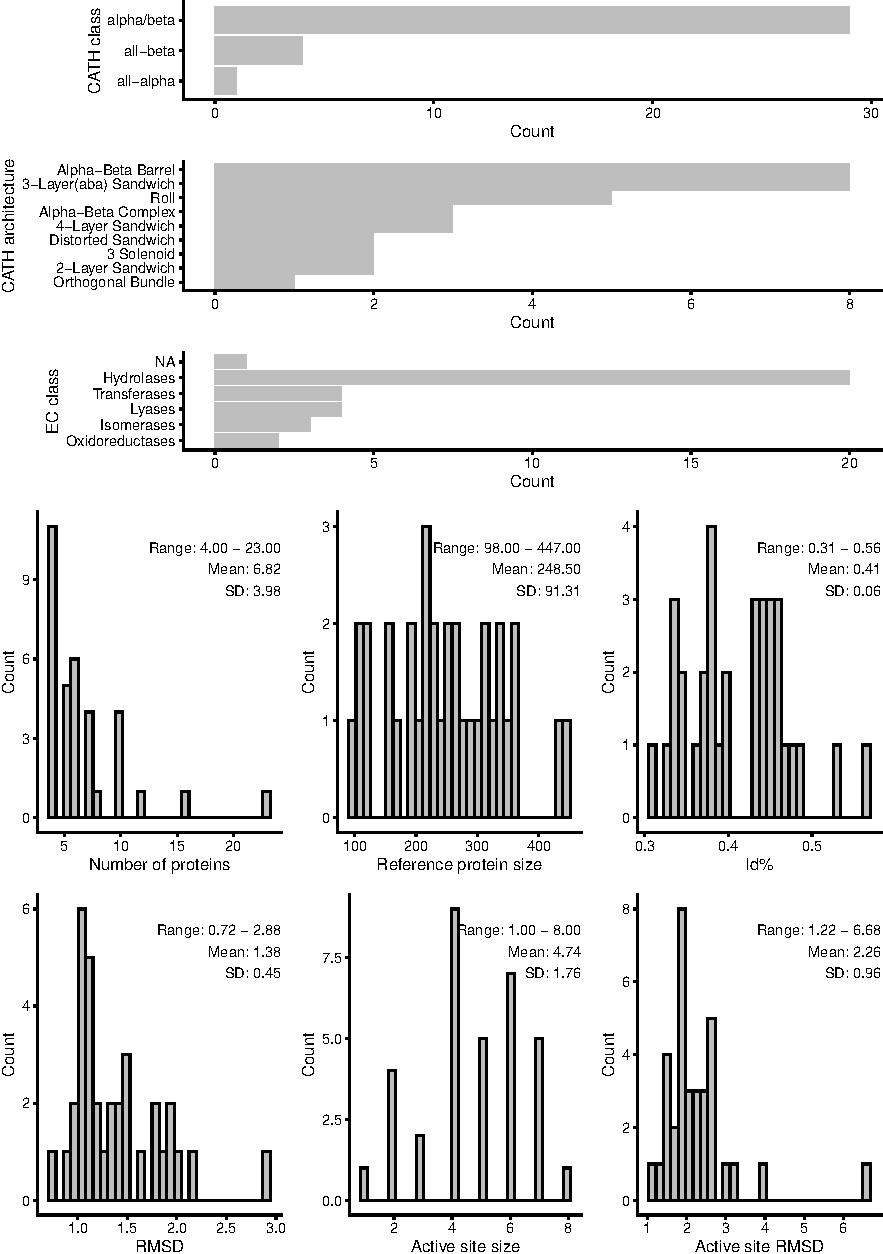
\includegraphics{supplementary_material_files/figure-latex/load_data_and_create_plot-1} 

}

\caption{Distribution of properties of dataset families.}\label{fig:load_data_and_create_plot}
\end{figure}

\clearpage

\clearpage

\hypertarget{correlation-between-flexibility-and-distance}{%
\section{Correlation between flexibility and
distance}\label{correlation-between-flexibility-and-distance}}

The following figure shows the distribution of spearman correlations
between flexibility (lRMSF) and distance to the active site (d) (panel
a). The correlation between these variables depends on the location of
the active site within the enzyme structure. In most cases active sites
are located in relatively rigid regions. Therefore, as one moves away
from the active site, not only distance increases but flexibility too,
which originates the correlation (panel b).

\begin{figure}

{\centering 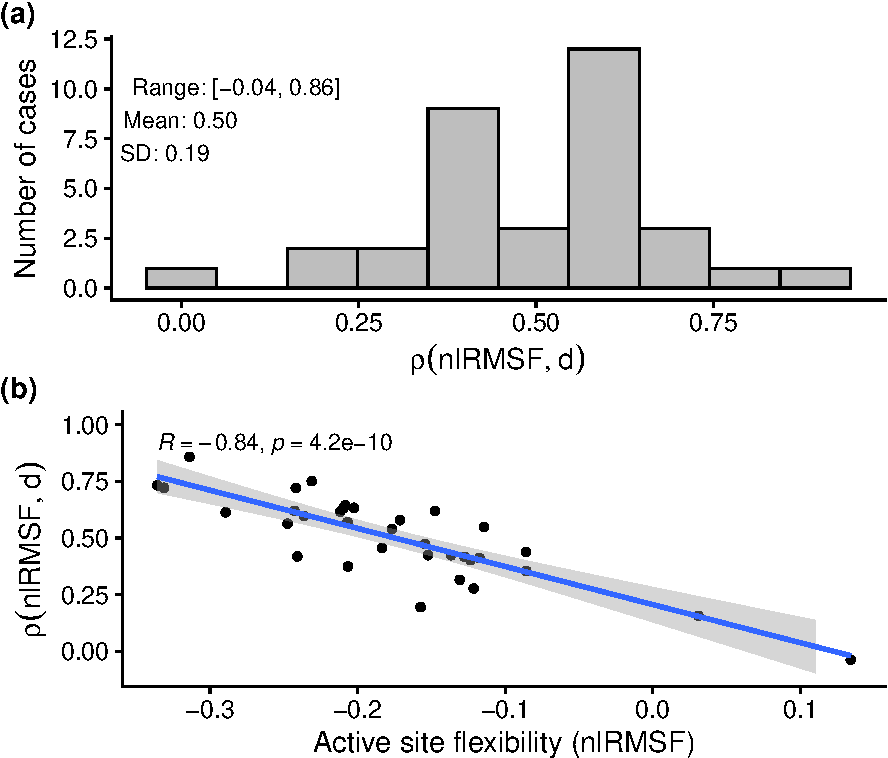
\includegraphics{supplementary_material_files/figure-latex/flex-dist correlation-1} 

}

\caption{Correlation betwen flexibility and distance.}\label{fig:flex-dist correlation}
\end{figure}

\clearpage

\clearpage

\hypertarget{family-by-family-analysis}{%
\section{Family by family analysis}\label{family-by-family-analysis}}

\hypertarget{figure-description}{%
\subsection{Figure Description}\label{figure-description}}

Each figure in this section represents a structural divergence analysis
for a specific enzyme family, identified by its MCSA ID.

Each figure is organized as follows:

Observed patterns: (a) Residue-specific structural divergence profile,
showing normalized log-RMSD (nlRMSD) across residues. (b) Relationship
between structural divergence (nlRMSD) and residue flexibility (nlRMSF).
(c) Relationship between structural divergence (nlRMSD) and distance
from the active site (d).

Model predictions vs.~observations: (d) Comparison of observed nlRMSD
profile with predictions from models M1, M2, and M12. (e) Flexibility
trends: observed data vs.~model predictions for nlRMSD vs.~nlRMSF. (f)
Distance trends: observed data vs.~model predictions for nlRMSD vs.~d.

Decomposition into flexibility and distance contributions: (g) Profile
of structural divergence decomposed into flexibility (s1) and distance
(s2) components. (h) Flexibility (s1) component of structural
divergence. (i) Distance (s2) component of structural divergence.

\clearpage
\begin{figure}[H]
\centering


\begin{center}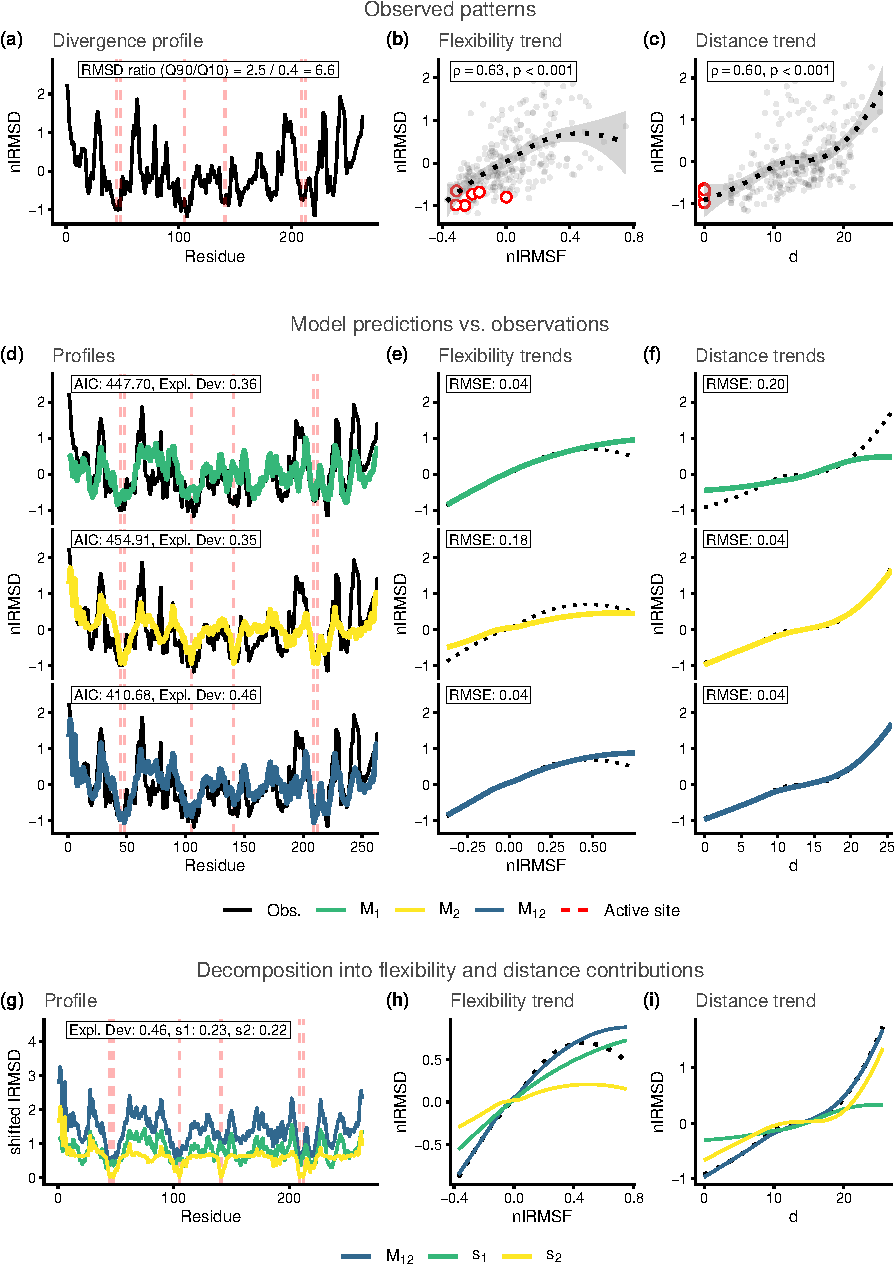
\includegraphics{supplementary_material_files/figure-latex/generate_figures-1} \end{center}

\caption{Structural divergence analysis for enzyme family MCSA ID: 2. Reference protein PDB ID: 1btl\_A.}
\end{figure}

\clearpage
\begin{figure}[H]
\centering


\begin{center}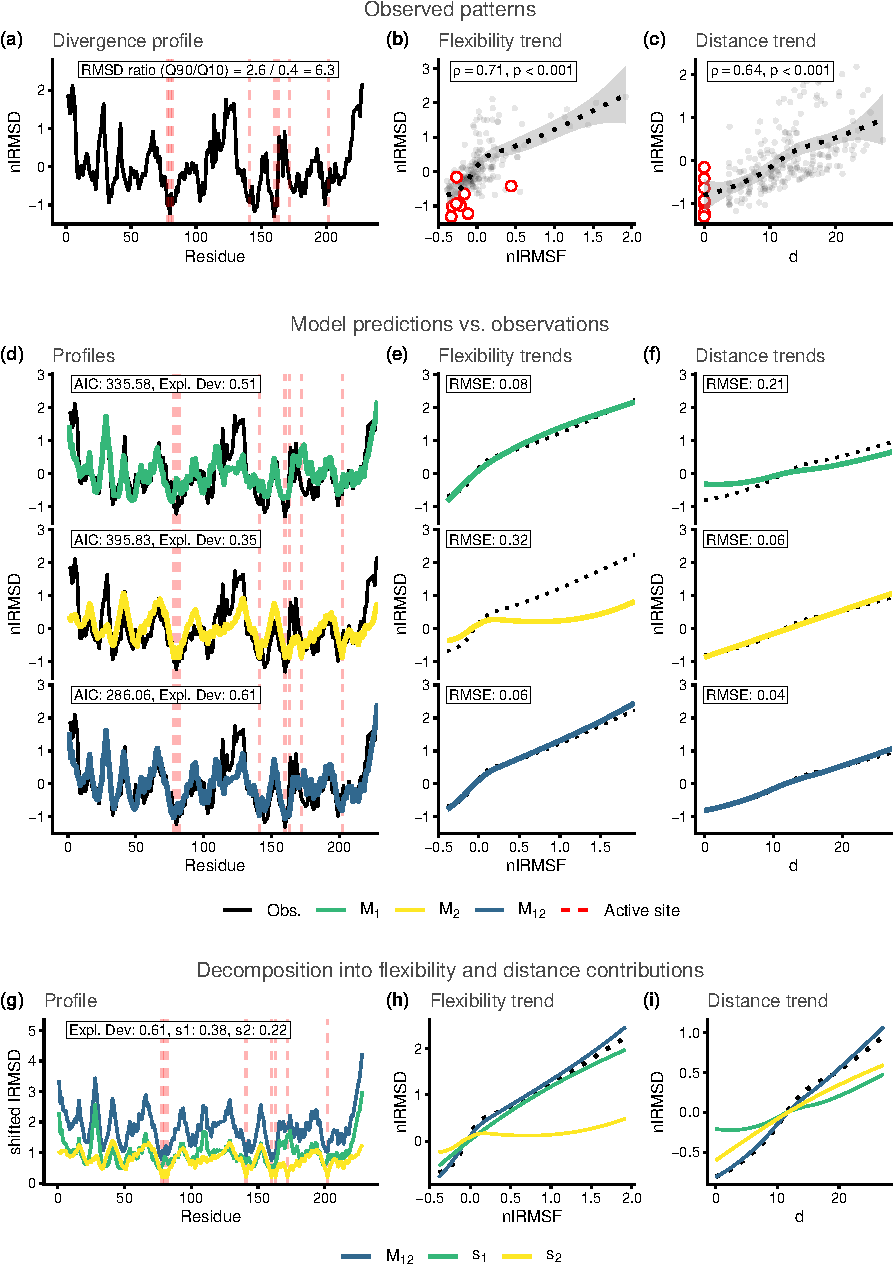
\includegraphics{supplementary_material_files/figure-latex/generate_figures-2} \end{center}

\caption{Structural divergence analysis for enzyme family MCSA ID: 15. Reference protein PDB ID: 1znb\_A.}
\end{figure}

\clearpage
\begin{figure}[H]
\centering


\begin{center}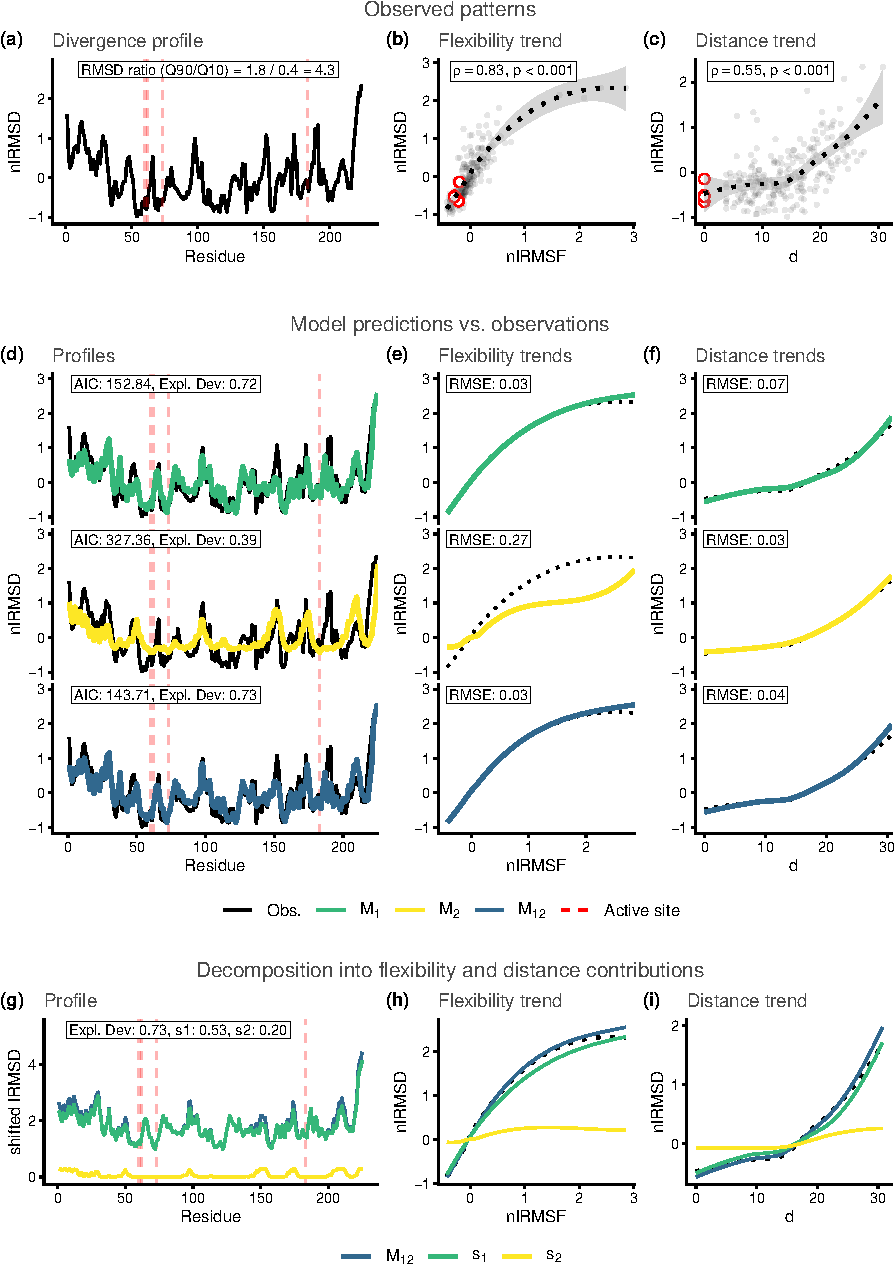
\includegraphics{supplementary_material_files/figure-latex/generate_figures-3} \end{center}

\caption{Structural divergence analysis for enzyme family MCSA ID: 71. Reference protein PDB ID: 1eug\_A.}
\end{figure}

\clearpage
\begin{figure}[H]
\centering


\begin{center}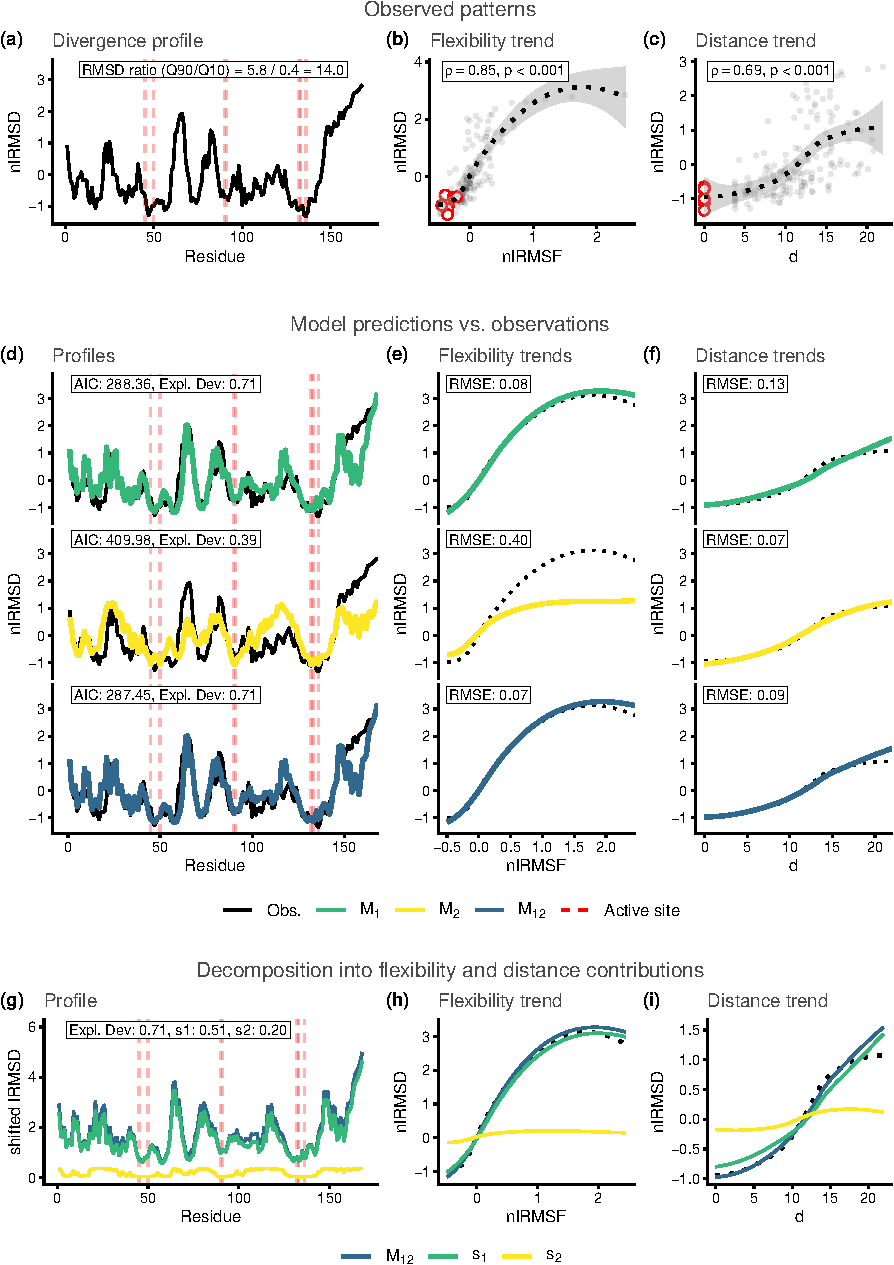
\includegraphics{supplementary_material_files/figure-latex/generate_figures-4} \end{center}

\caption{Structural divergence analysis for enzyme family MCSA ID: 98. Reference protein PDB ID: 1bsz\_C.}
\end{figure}

\clearpage
\begin{figure}[H]
\centering


\begin{center}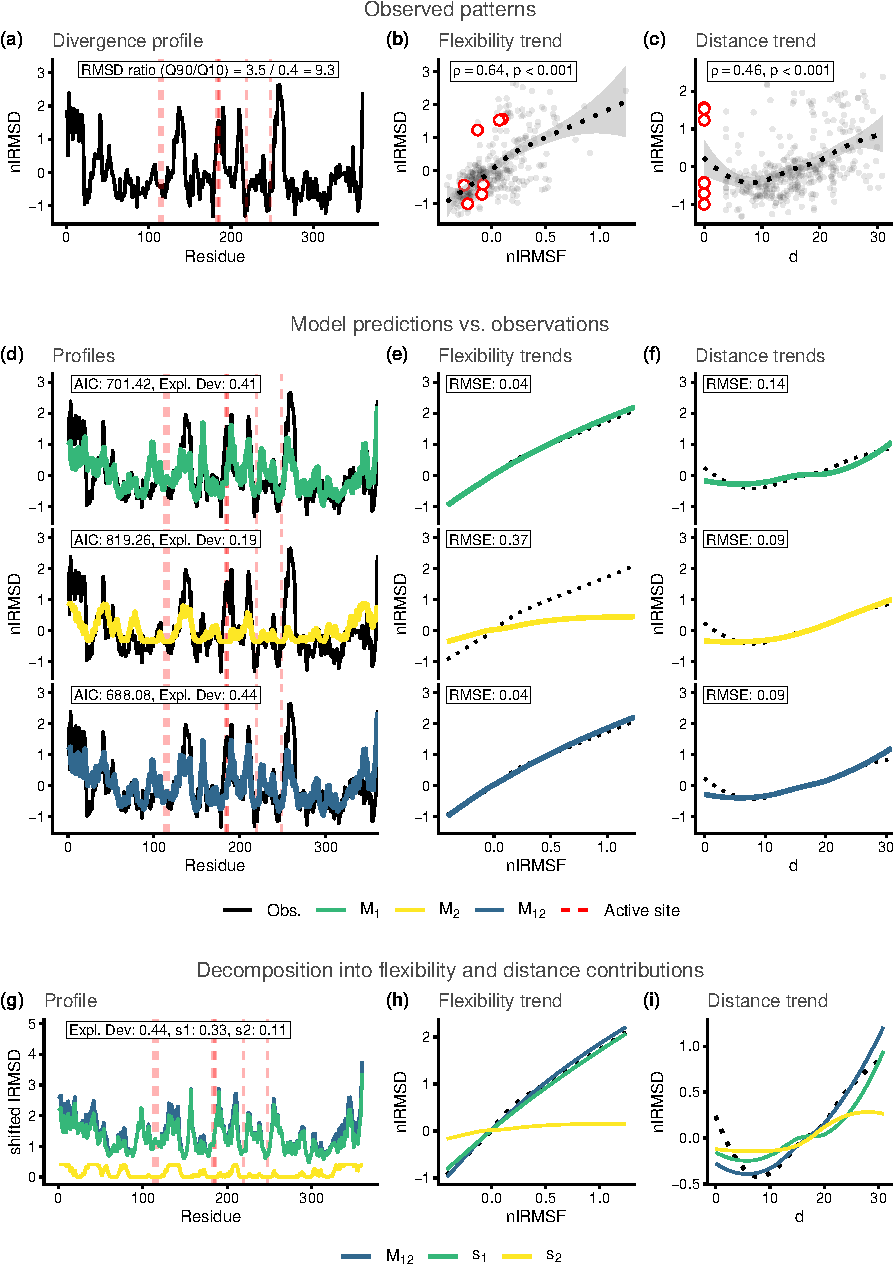
\includegraphics{supplementary_material_files/figure-latex/generate_figures-5} \end{center}

\caption{Structural divergence analysis for enzyme family MCSA ID: 109. Reference protein PDB ID: 1d3g\_A.}
\end{figure}

\clearpage
\begin{figure}[H]
\centering


\begin{center}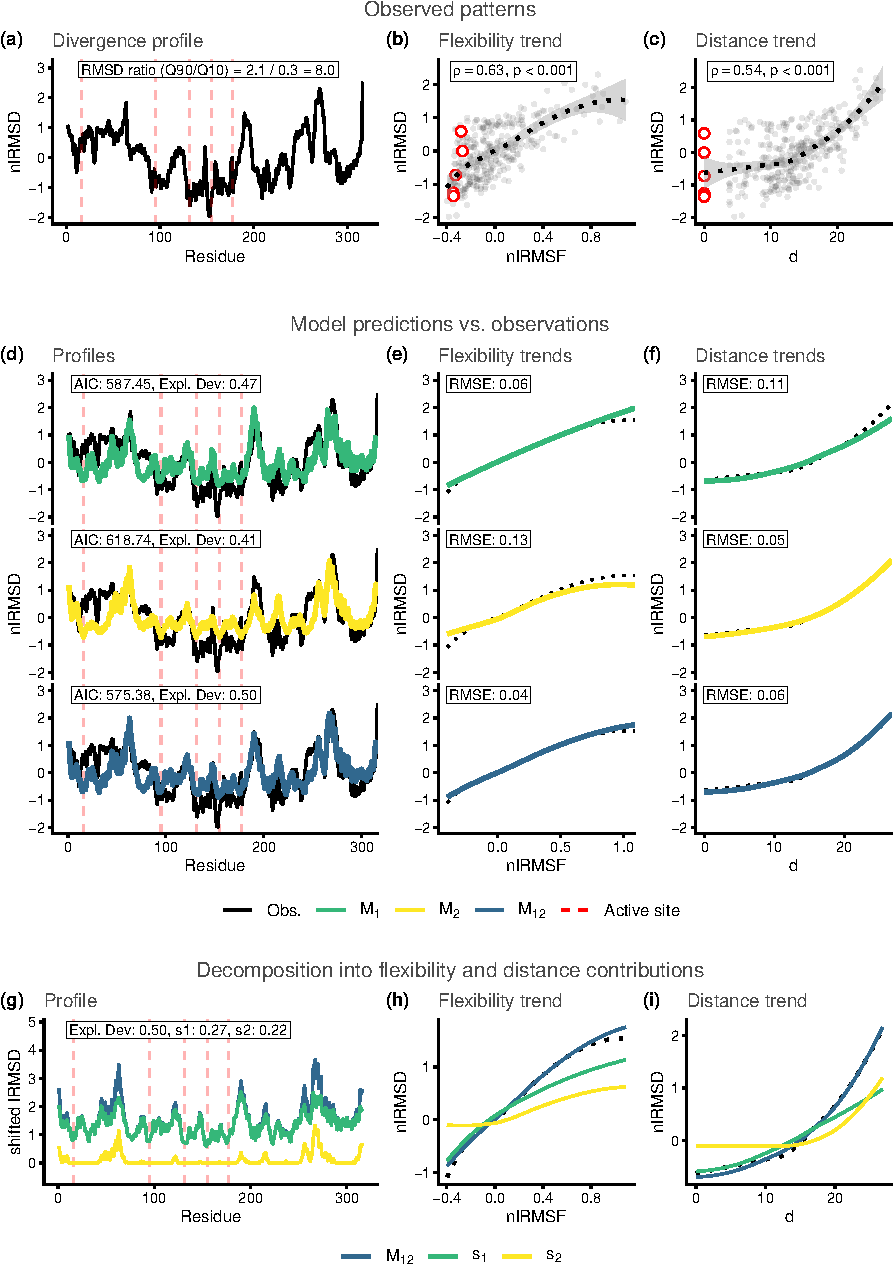
\includegraphics{supplementary_material_files/figure-latex/generate_figures-6} \end{center}

\caption{Structural divergence analysis for enzyme family MCSA ID: 148. Reference protein PDB ID: 1onr\_A.}
\end{figure}

\clearpage
\begin{figure}[H]
\centering


\begin{center}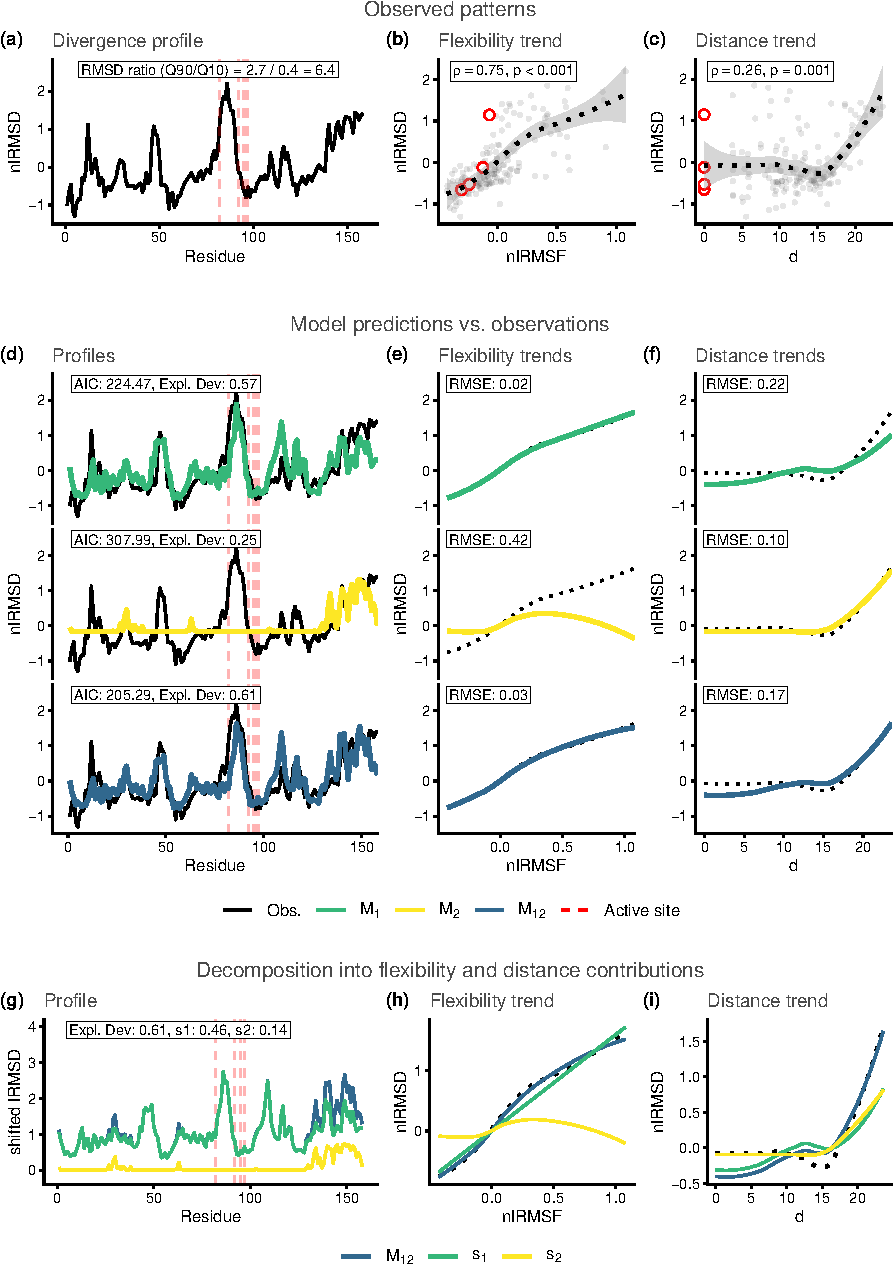
\includegraphics{supplementary_material_files/figure-latex/generate_figures-7} \end{center}

\caption{Structural divergence analysis for enzyme family MCSA ID: 151. Reference protein PDB ID: 1q0n\_A.}
\end{figure}

\clearpage
\begin{figure}[H]
\centering


\begin{center}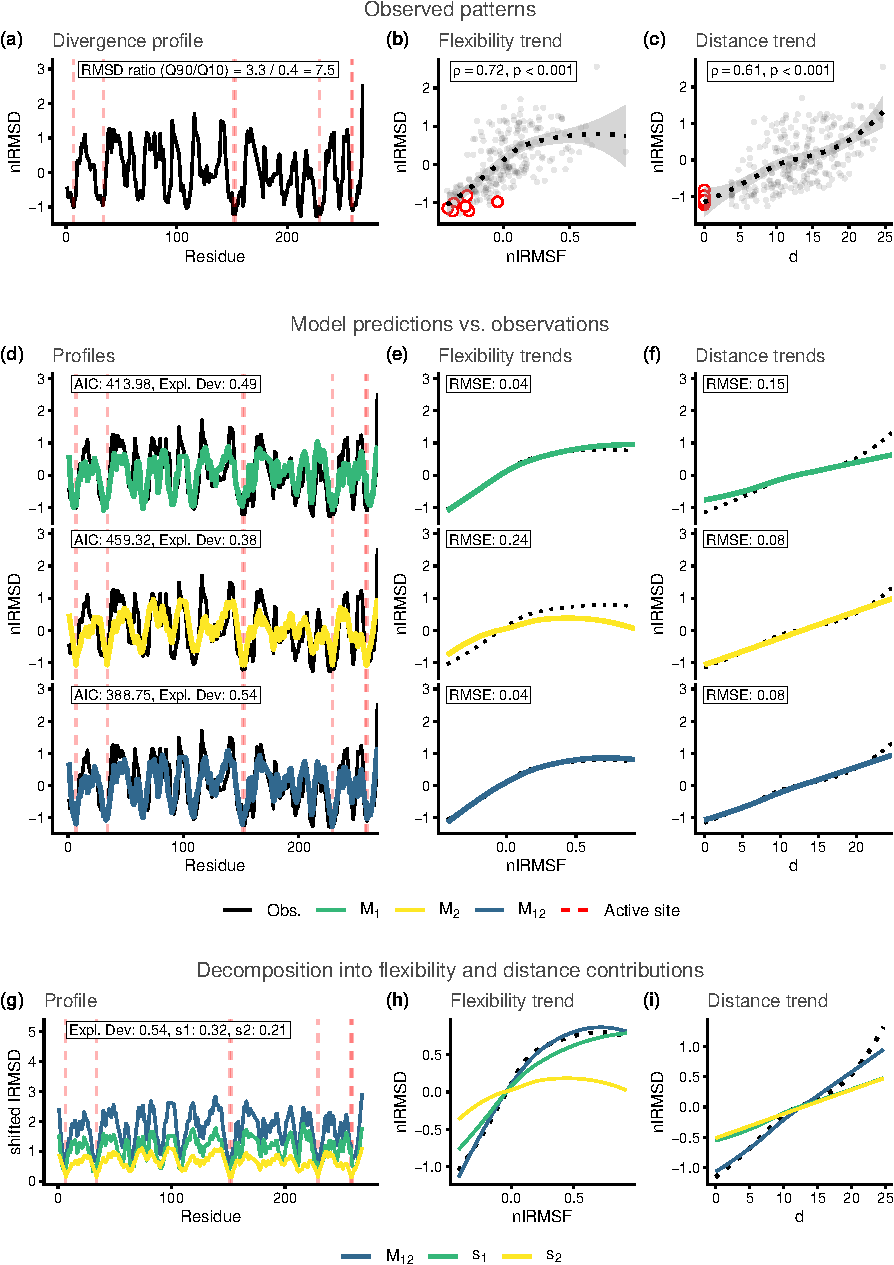
\includegraphics{supplementary_material_files/figure-latex/generate_figures-8} \end{center}

\caption{Structural divergence analysis for enzyme family MCSA ID: 160. Reference protein PDB ID: 1ako\_A.}
\end{figure}

\clearpage
\begin{figure}[H]
\centering


\begin{center}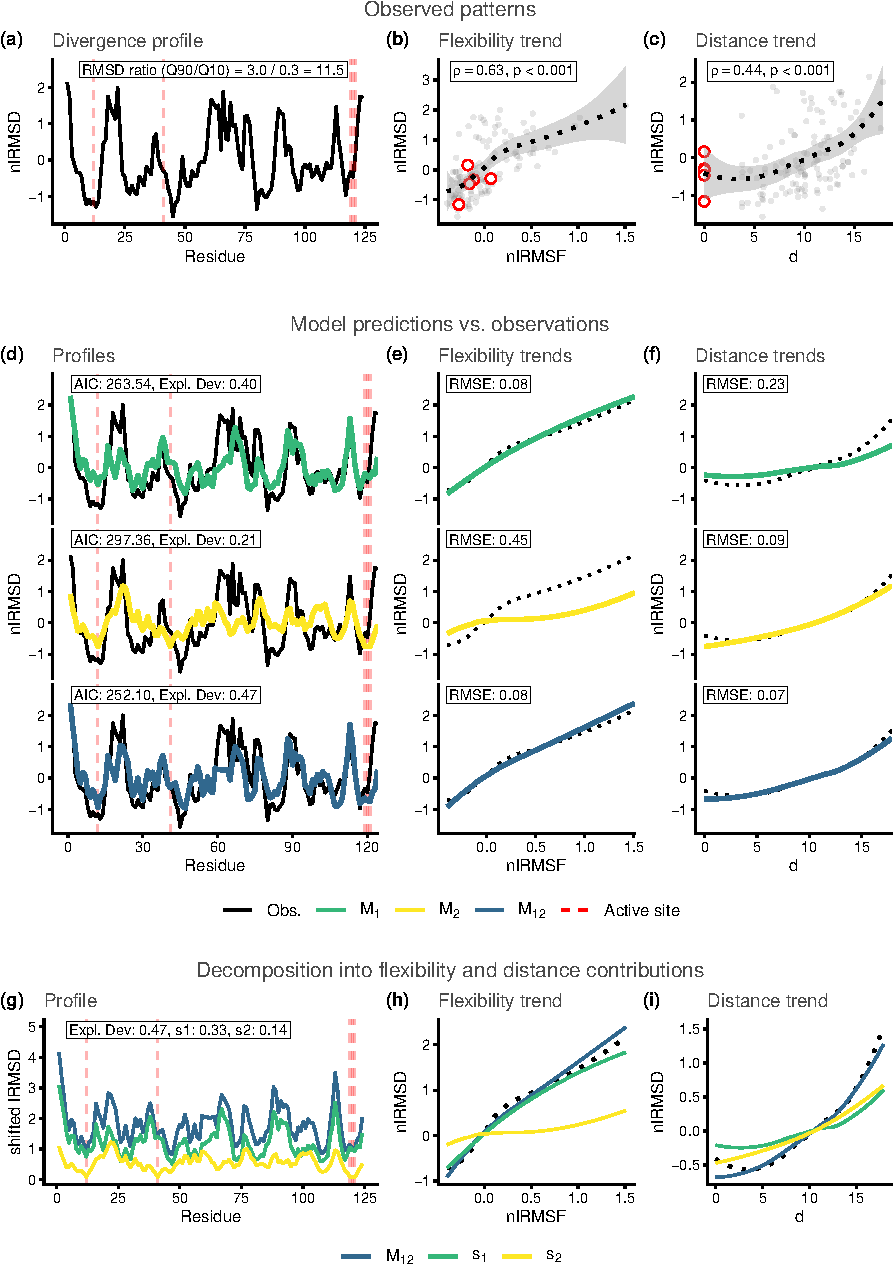
\includegraphics{supplementary_material_files/figure-latex/generate_figures-9} \end{center}

\caption{Structural divergence analysis for enzyme family MCSA ID: 164. Reference protein PDB ID: 1ruv\_A.}
\end{figure}

\clearpage
\begin{figure}[H]
\centering


\begin{center}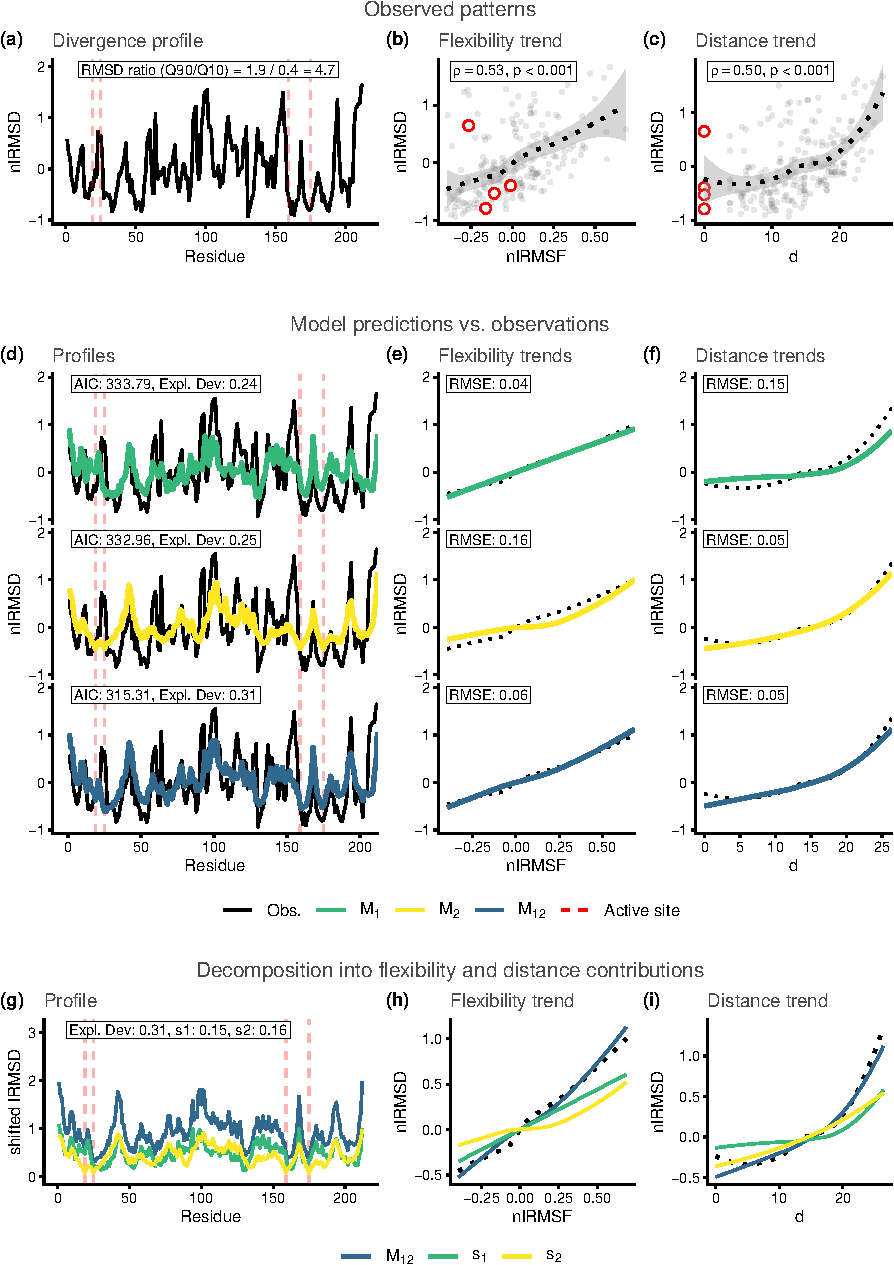
\includegraphics{supplementary_material_files/figure-latex/generate_figures-10} \end{center}

\caption{Structural divergence analysis for enzyme family MCSA ID: 174. Reference protein PDB ID: 9pap\_A.}
\end{figure}

\clearpage
\begin{figure}[H]
\centering


\begin{center}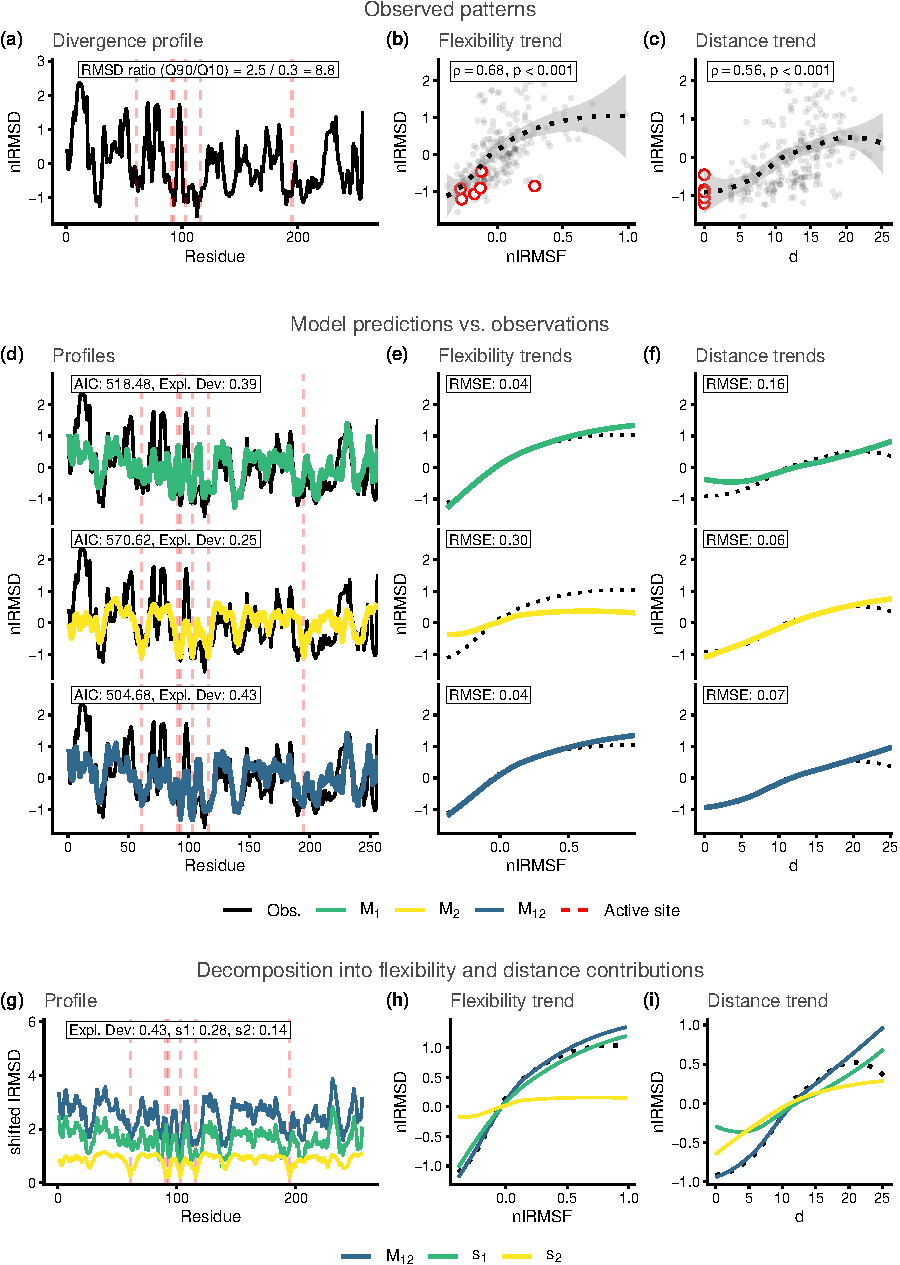
\includegraphics{supplementary_material_files/figure-latex/generate_figures-11} \end{center}

\caption{Structural divergence analysis for enzyme family MCSA ID: 216. Reference protein PDB ID: 1ca2\_A.}
\end{figure}

\clearpage
\begin{figure}[H]
\centering


\begin{center}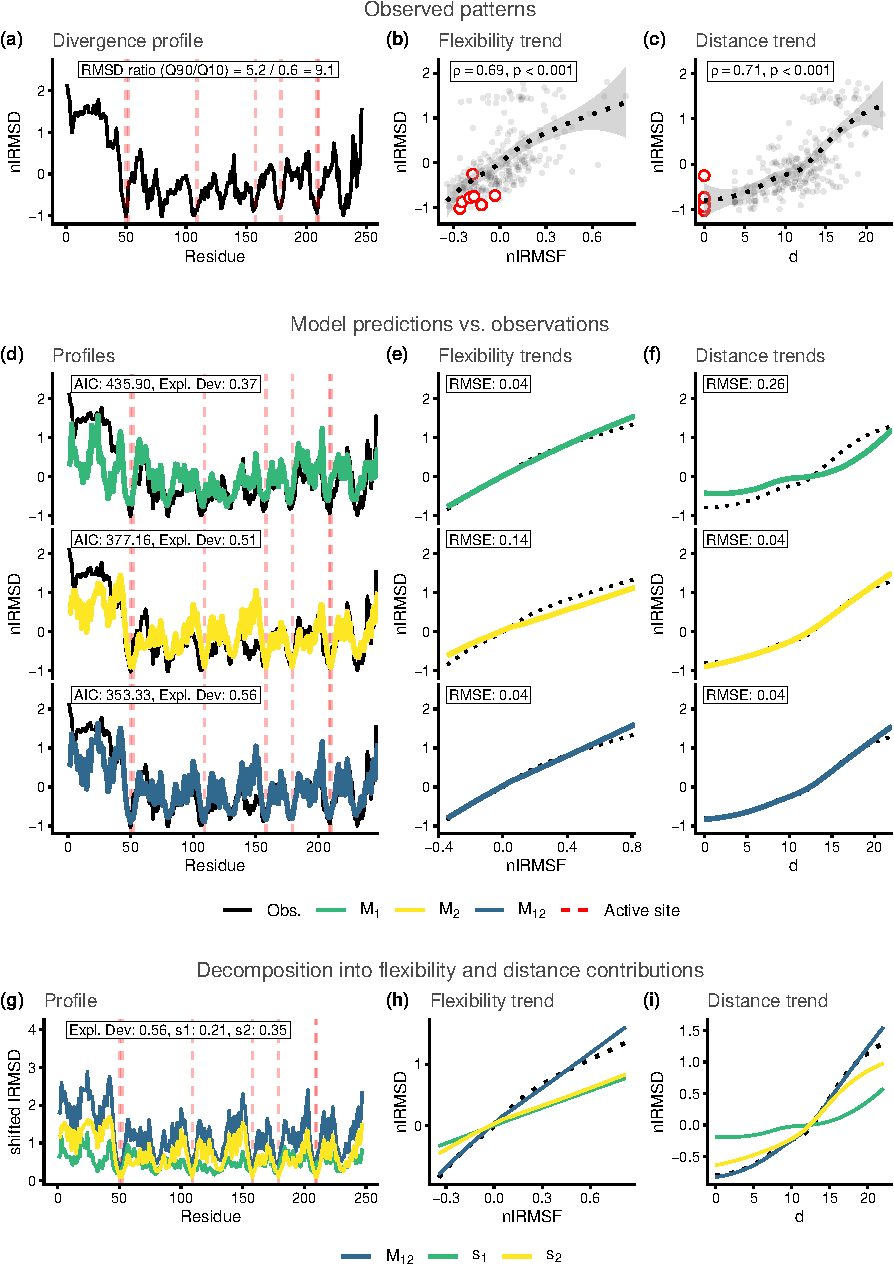
\includegraphics{supplementary_material_files/figure-latex/generate_figures-12} \end{center}

\caption{Structural divergence analysis for enzyme family MCSA ID: 252. Reference protein PDB ID: 1igs\_A.}
\end{figure}

\clearpage
\begin{figure}[H]
\centering


\begin{center}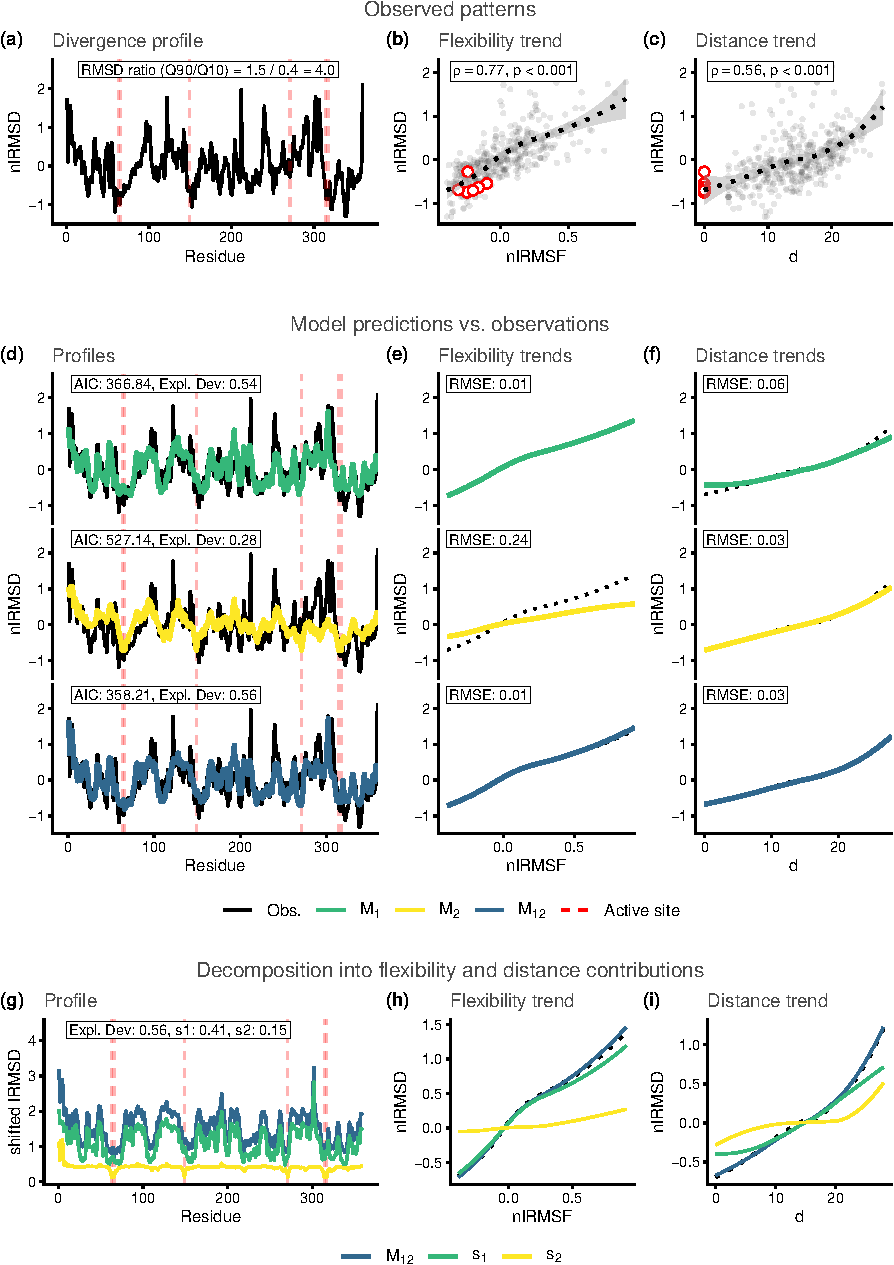
\includegraphics{supplementary_material_files/figure-latex/generate_figures-13} \end{center}

\caption{Structural divergence analysis for enzyme family MCSA ID: 257. Reference protein PDB ID: 1xx2\_A.}
\end{figure}

\clearpage
\begin{figure}[H]
\centering


\begin{center}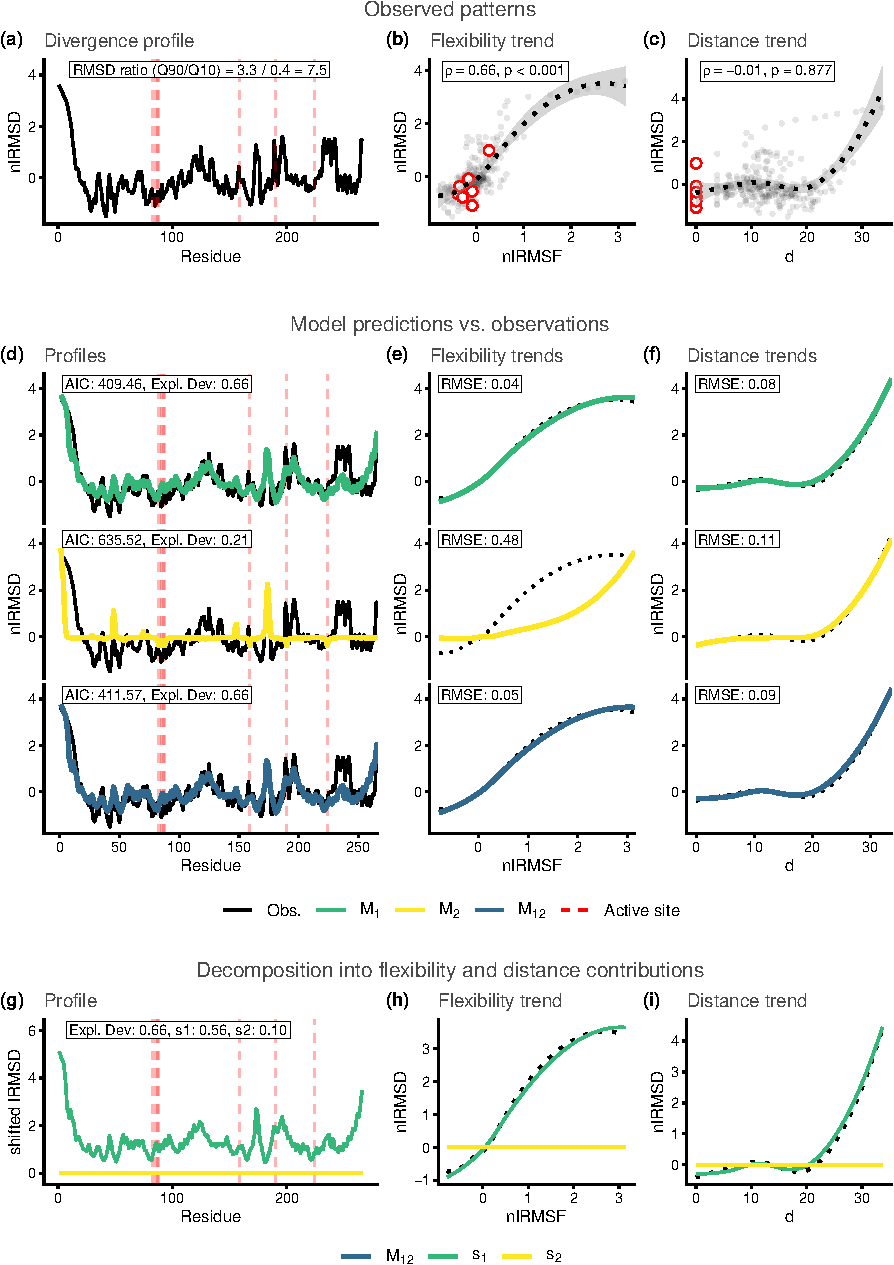
\includegraphics{supplementary_material_files/figure-latex/generate_figures-14} \end{center}

\caption{Structural divergence analysis for enzyme family MCSA ID: 258. Reference protein PDB ID: 1sml\_A.}
\end{figure}

\clearpage
\begin{figure}[H]
\centering


\begin{center}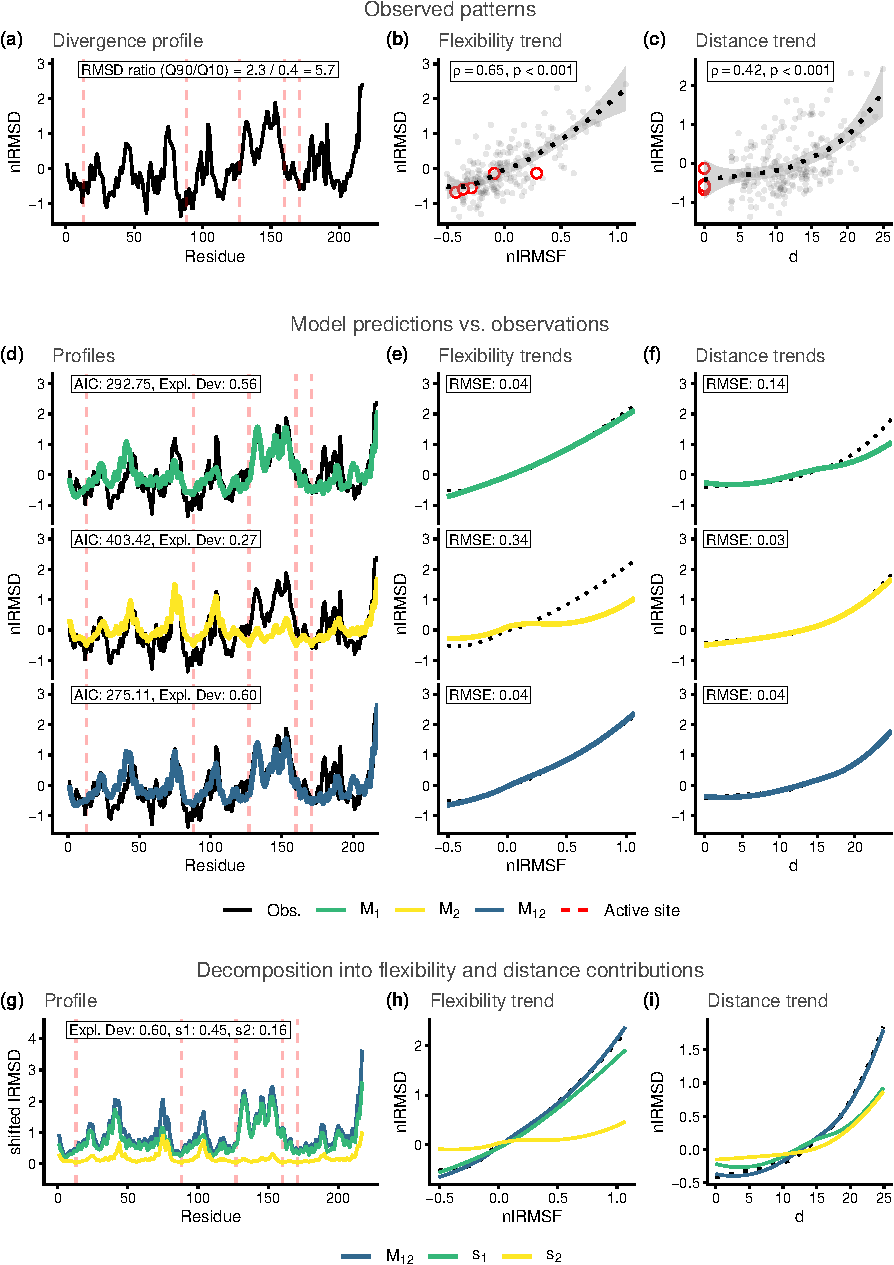
\includegraphics{supplementary_material_files/figure-latex/generate_figures-15} \end{center}

\caption{Structural divergence analysis for enzyme family MCSA ID: 290. Reference protein PDB ID: 1zio\_A.}
\end{figure}

\clearpage
\begin{figure}[H]
\centering


\begin{center}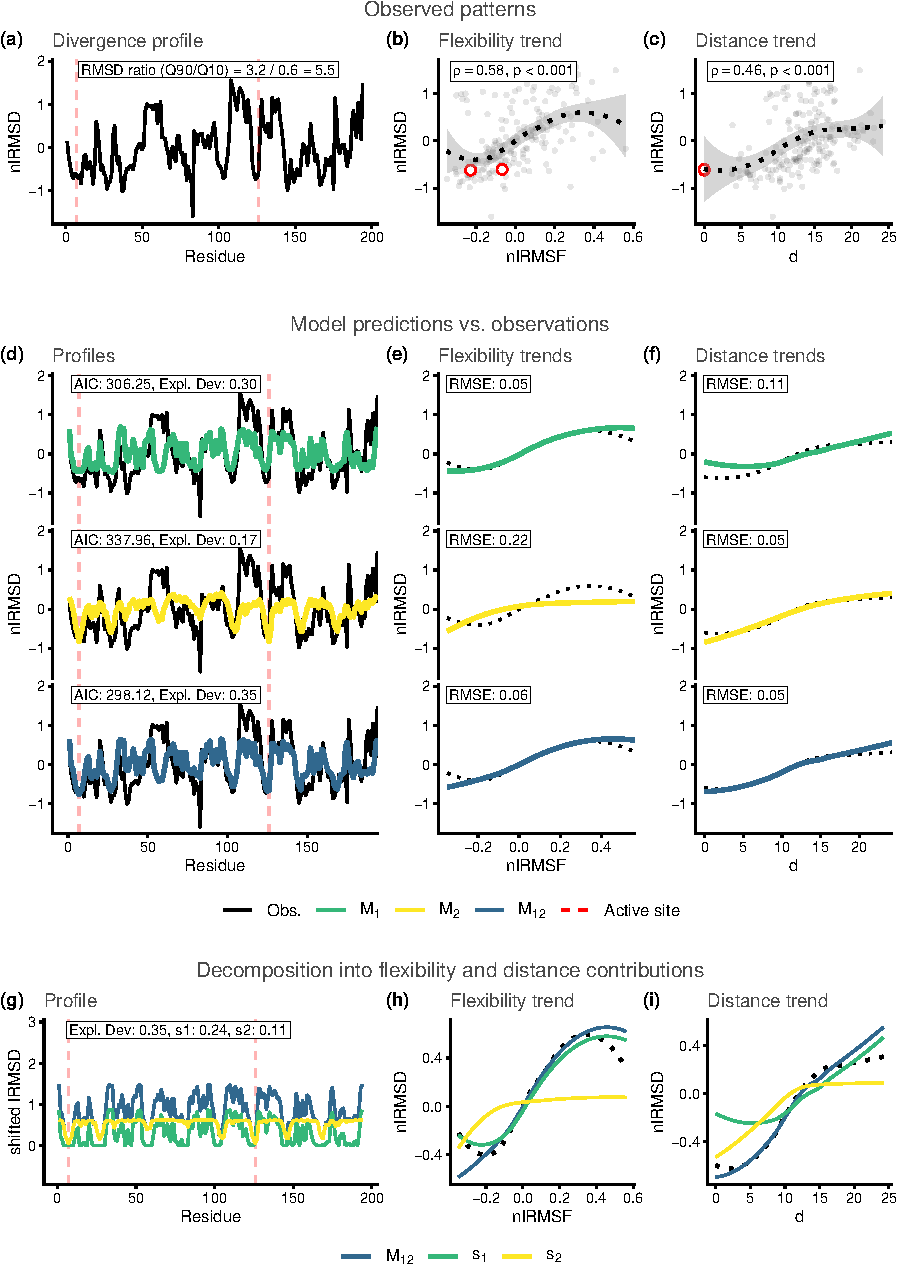
\includegraphics{supplementary_material_files/figure-latex/generate_figures-16} \end{center}

\caption{Structural divergence analysis for enzyme family MCSA ID: 328. Reference protein PDB ID: 1lbm\_A.}
\end{figure}

\clearpage
\begin{figure}[H]
\centering


\begin{center}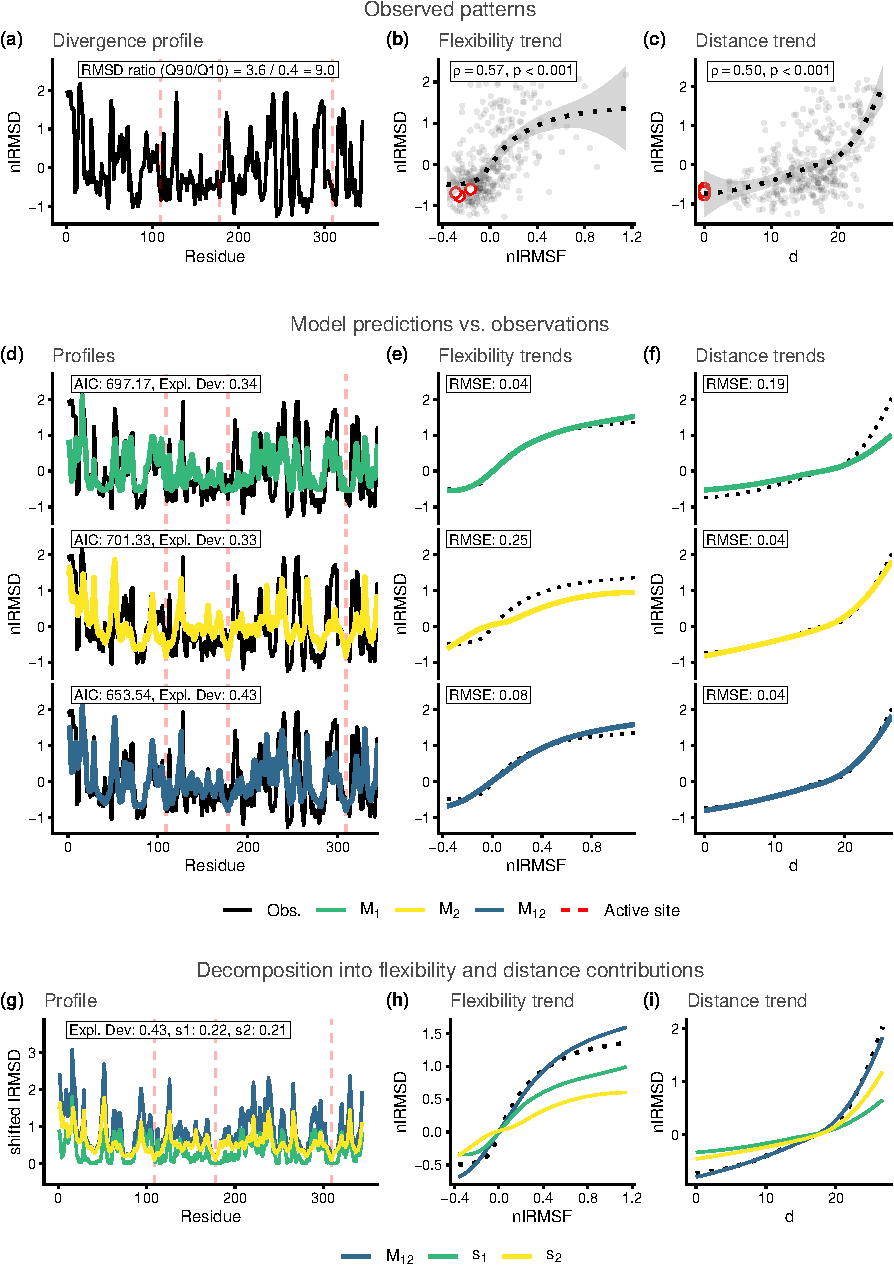
\includegraphics{supplementary_material_files/figure-latex/generate_figures-17} \end{center}

\caption{Structural divergence analysis for enzyme family MCSA ID: 351. Reference protein PDB ID: 1snz\_A.}
\end{figure}

\clearpage
\begin{figure}[H]
\centering


\begin{center}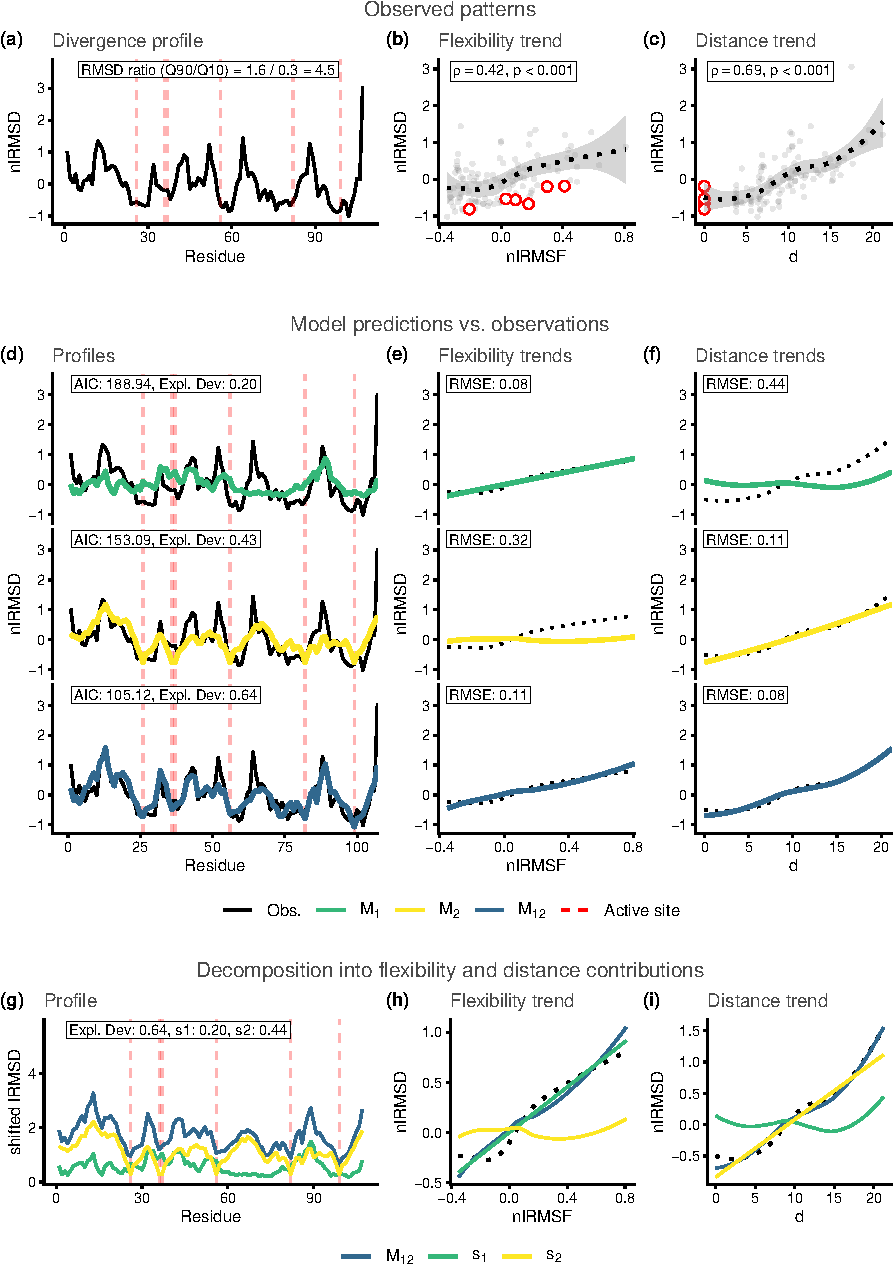
\includegraphics{supplementary_material_files/figure-latex/generate_figures-18} \end{center}

\caption{Structural divergence analysis for enzyme family MCSA ID: 362. Reference protein PDB ID: 1d6o\_A.}
\end{figure}

\clearpage
\begin{figure}[H]
\centering


\begin{center}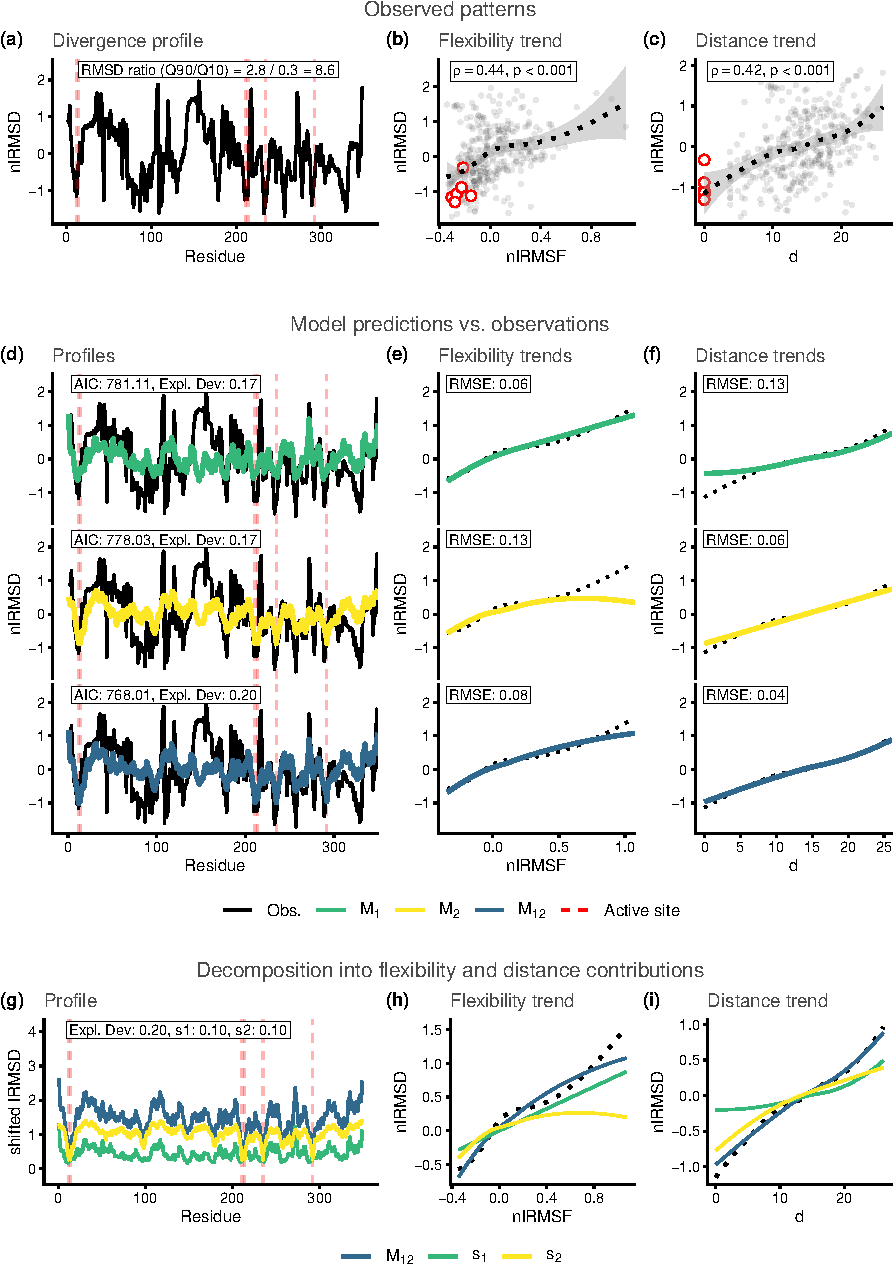
\includegraphics{supplementary_material_files/figure-latex/generate_figures-19} \end{center}

\caption{Structural divergence analysis for enzyme family MCSA ID: 376. Reference protein PDB ID: 1a4l\_A.}
\end{figure}

\clearpage
\begin{figure}[H]
\centering


\begin{center}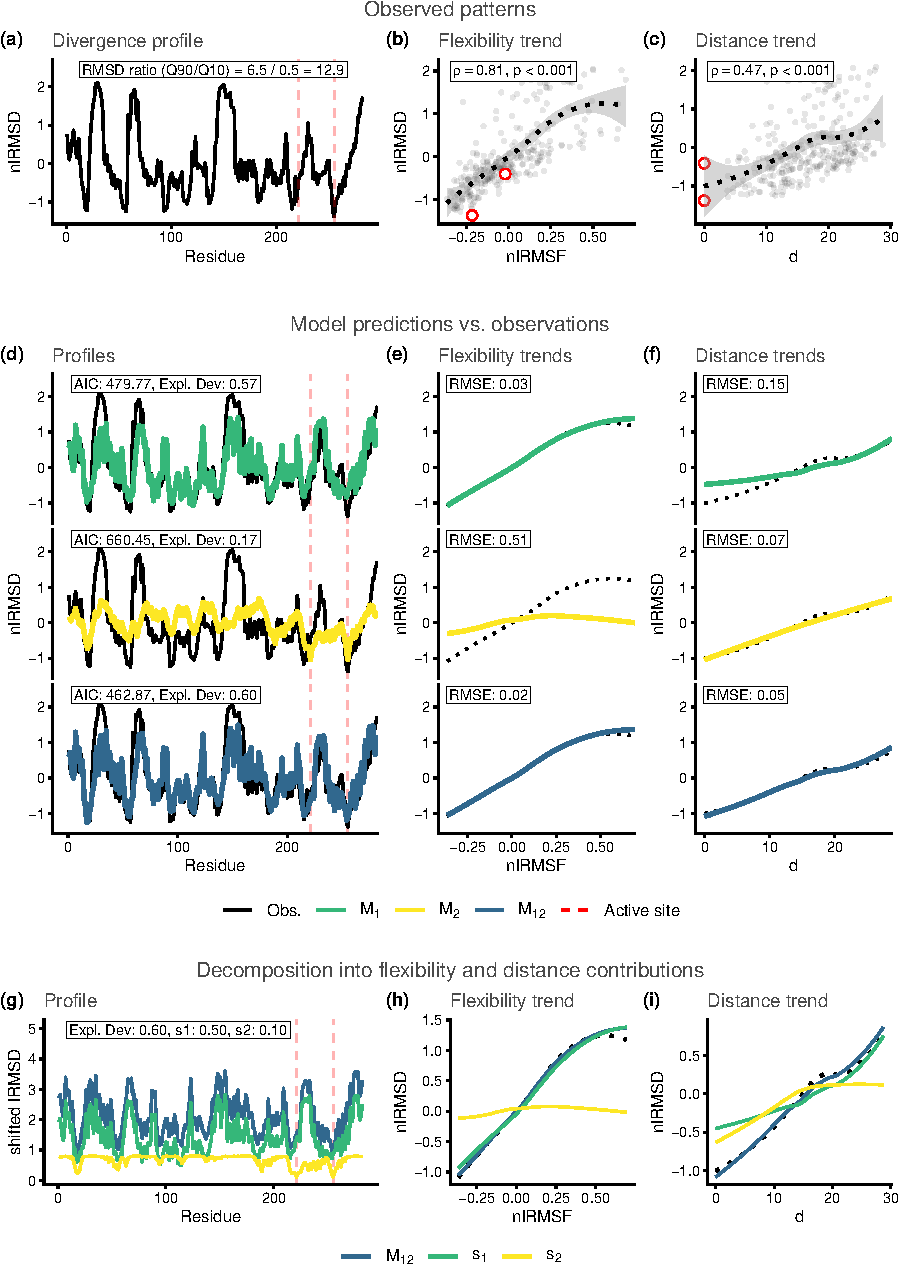
\includegraphics{supplementary_material_files/figure-latex/generate_figures-20} \end{center}

\caption{Structural divergence analysis for enzyme family MCSA ID: 394. Reference protein PDB ID: 1aj0\_A.}
\end{figure}

\clearpage
\begin{figure}[H]
\centering


\begin{center}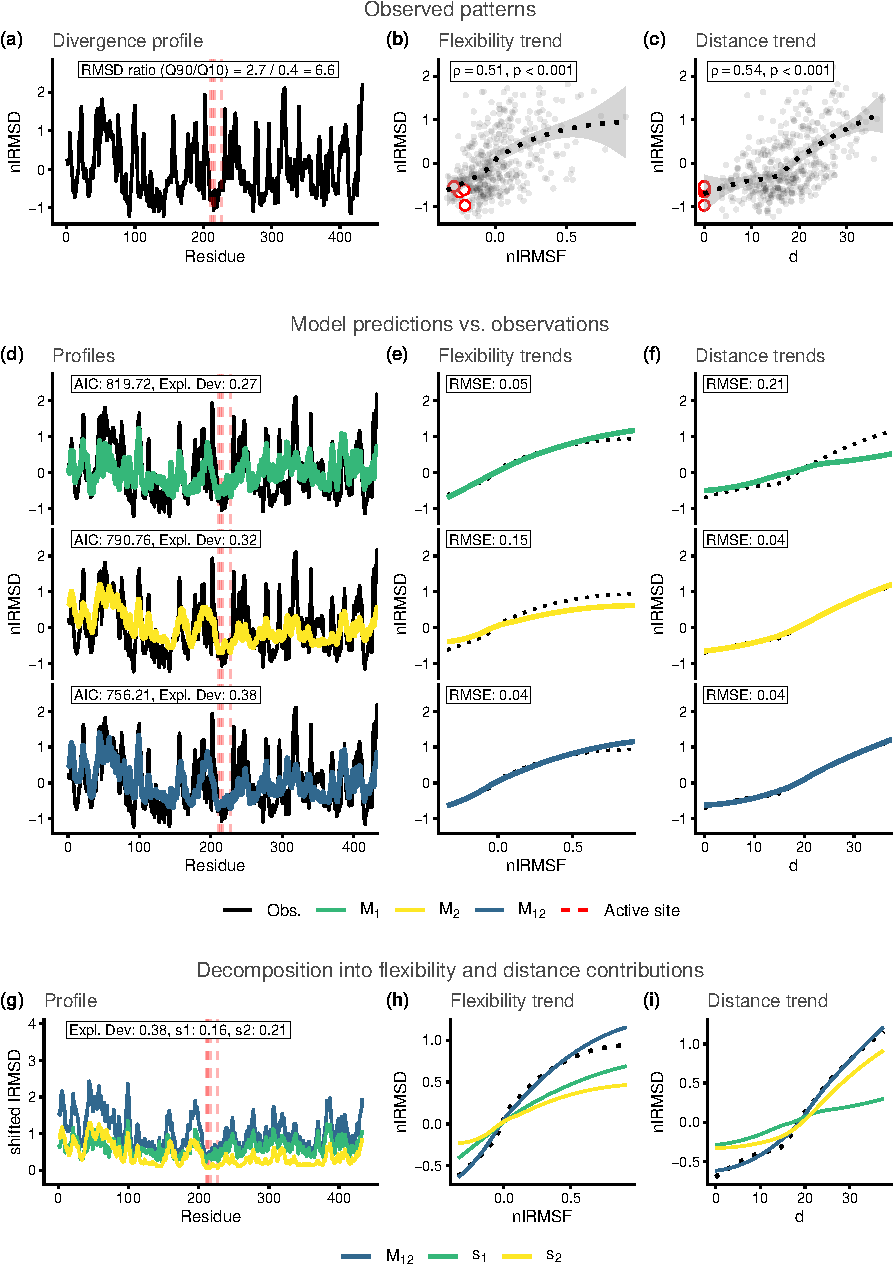
\includegraphics{supplementary_material_files/figure-latex/generate_figures-21} \end{center}

\caption{Structural divergence analysis for enzyme family MCSA ID: 444. Reference protein PDB ID: 1cel\_A.}
\end{figure}

\clearpage
\begin{figure}[H]
\centering


\begin{center}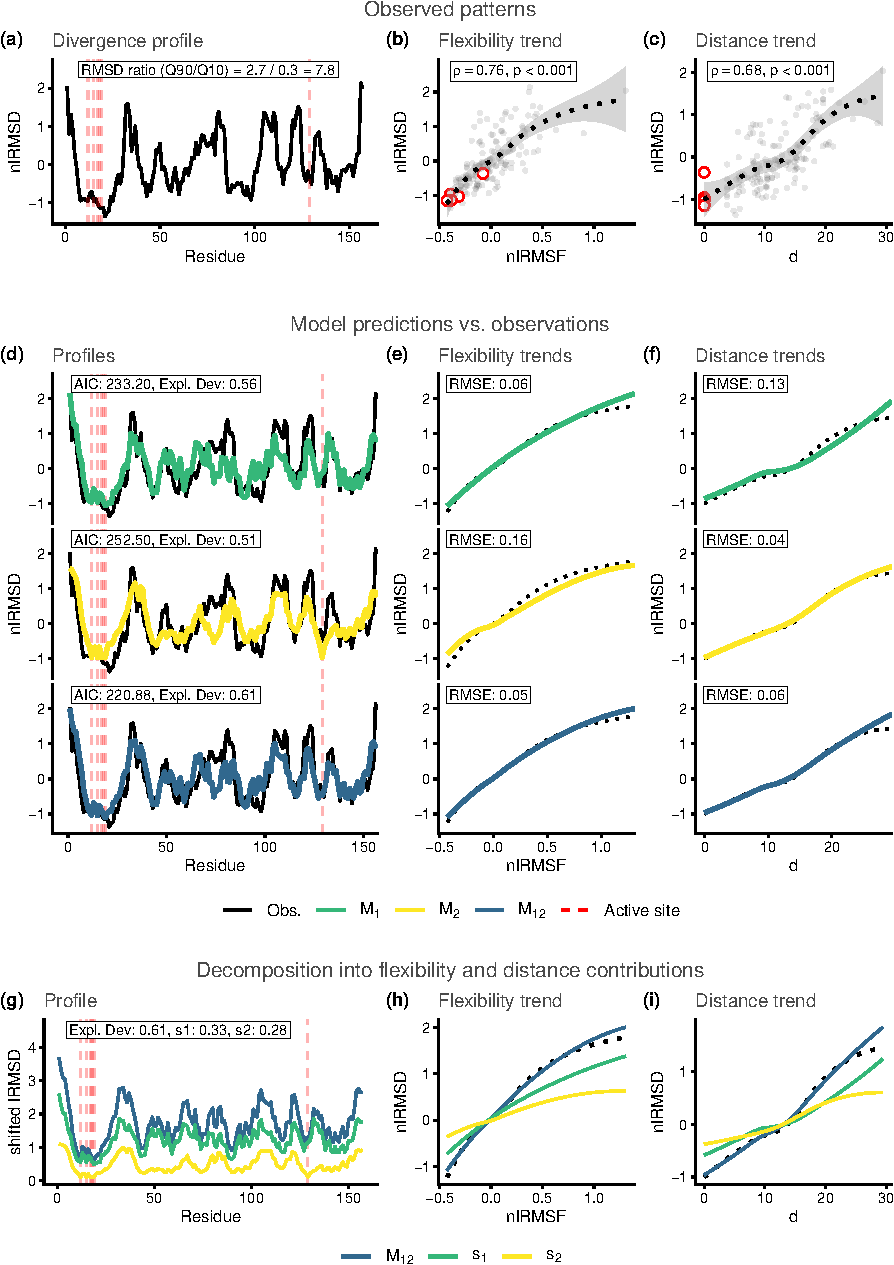
\includegraphics{supplementary_material_files/figure-latex/generate_figures-22} \end{center}

\caption{Structural divergence analysis for enzyme family MCSA ID: 462. Reference protein PDB ID: 1pnt\_A.}
\end{figure}

\clearpage
\begin{figure}[H]
\centering


\begin{center}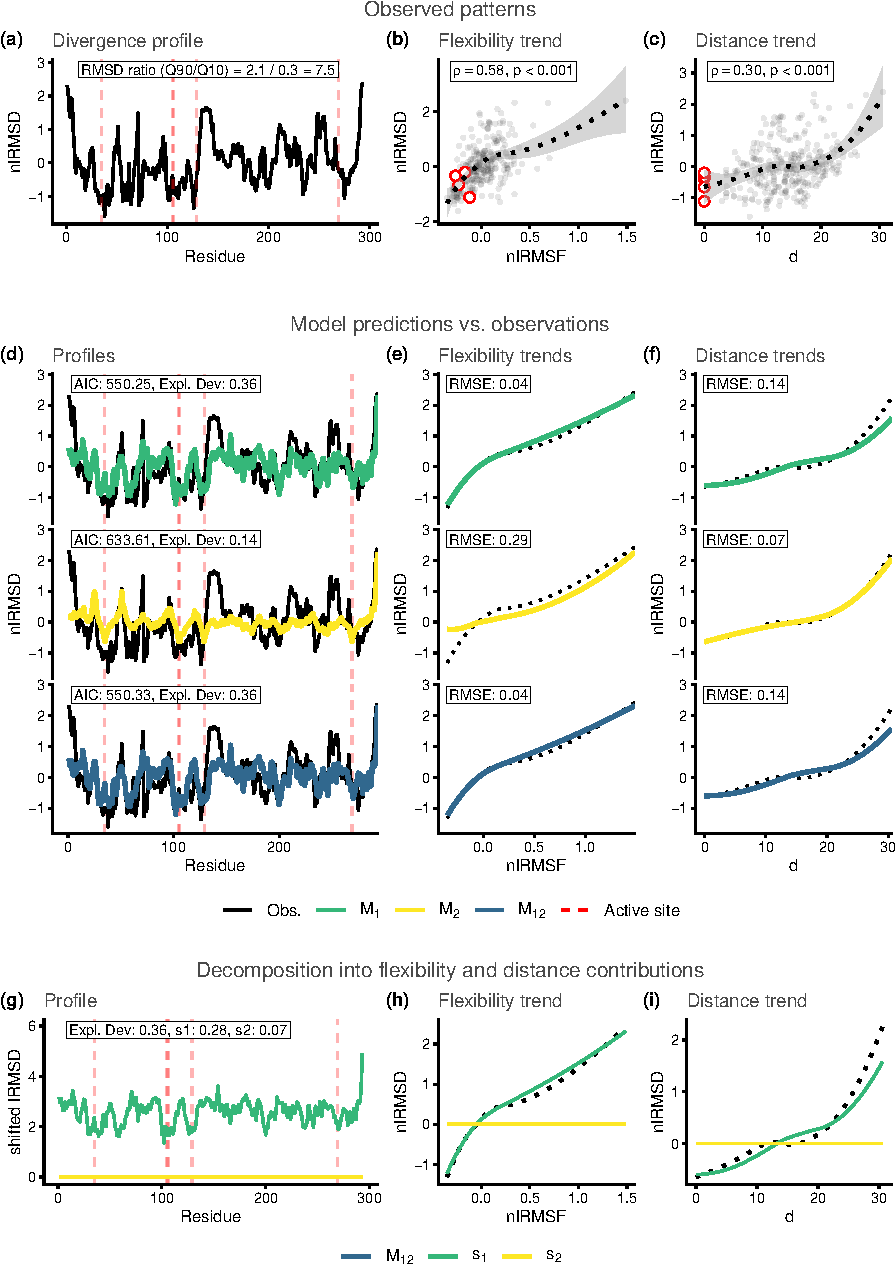
\includegraphics{supplementary_material_files/figure-latex/generate_figures-23} \end{center}

\caption{Structural divergence analysis for enzyme family MCSA ID: 467. Reference protein PDB ID: 1cv2\_A.}
\end{figure}

\clearpage
\begin{figure}[H]
\centering


\begin{center}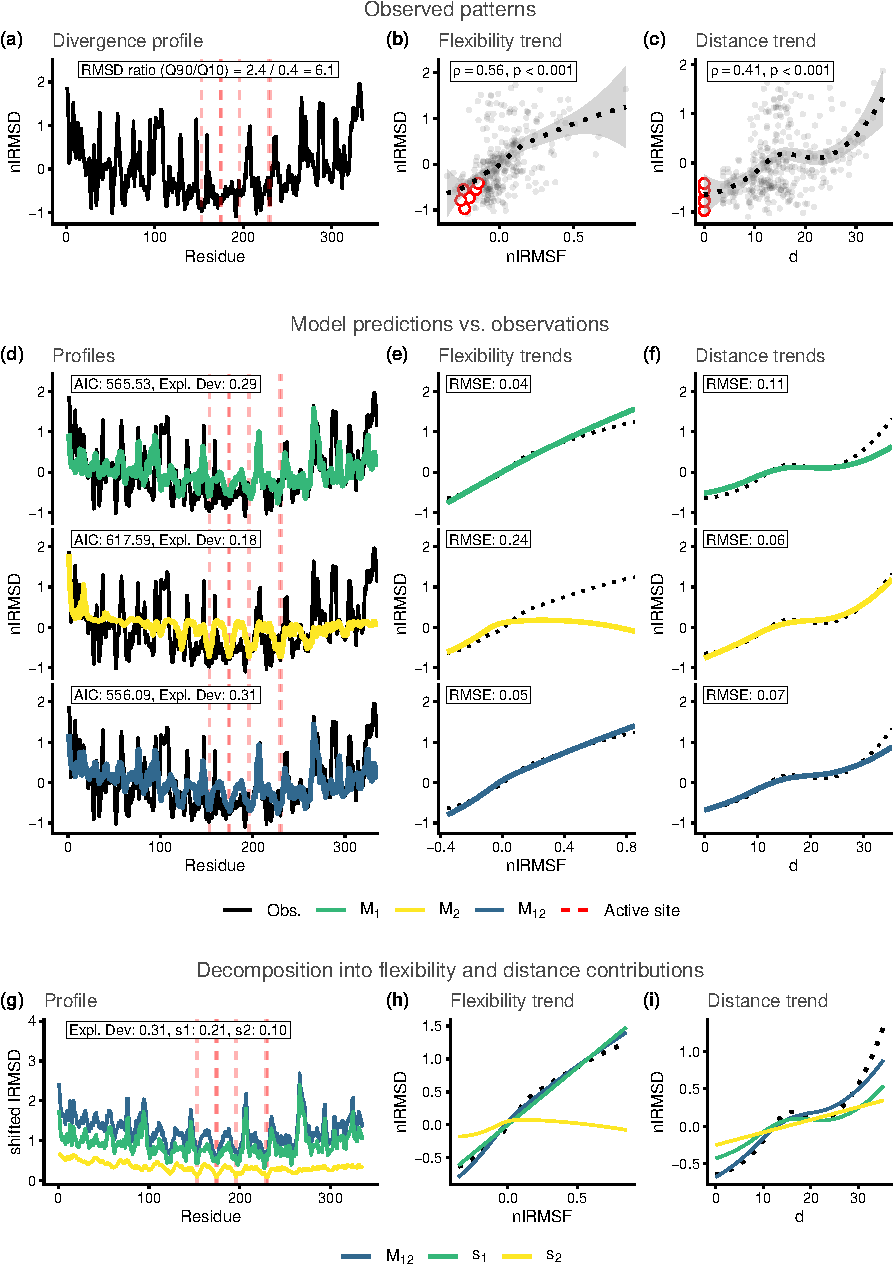
\includegraphics{supplementary_material_files/figure-latex/generate_figures-24} \end{center}

\caption{Structural divergence analysis for enzyme family MCSA ID: 480. Reference protein PDB ID: 1czf\_A.}
\end{figure}

\clearpage
\begin{figure}[H]
\centering


\begin{center}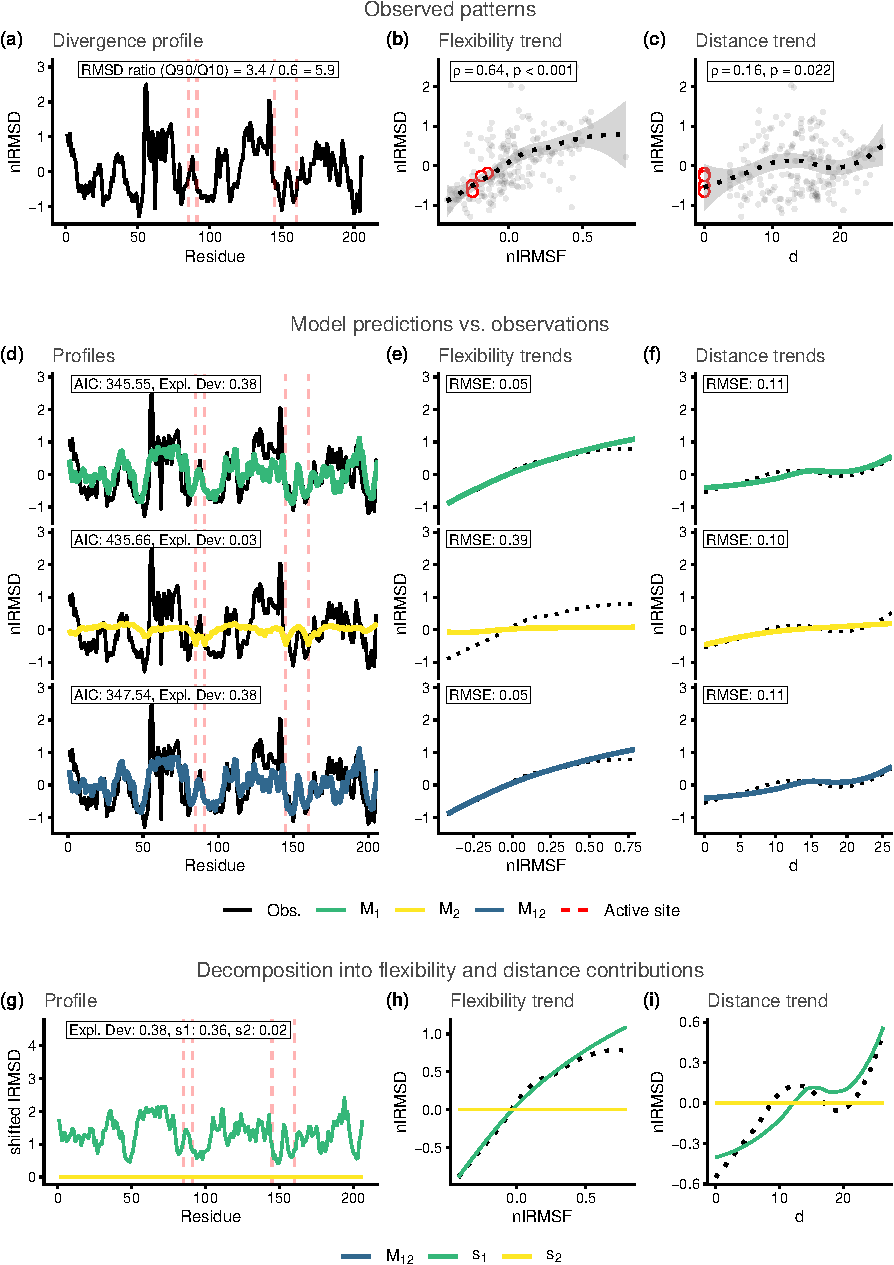
\includegraphics{supplementary_material_files/figure-latex/generate_figures-25} \end{center}

\caption{Structural divergence analysis for enzyme family MCSA ID: 597. Reference protein PDB ID: 1uch\_A.}
\end{figure}

\clearpage
\begin{figure}[H]
\centering


\begin{center}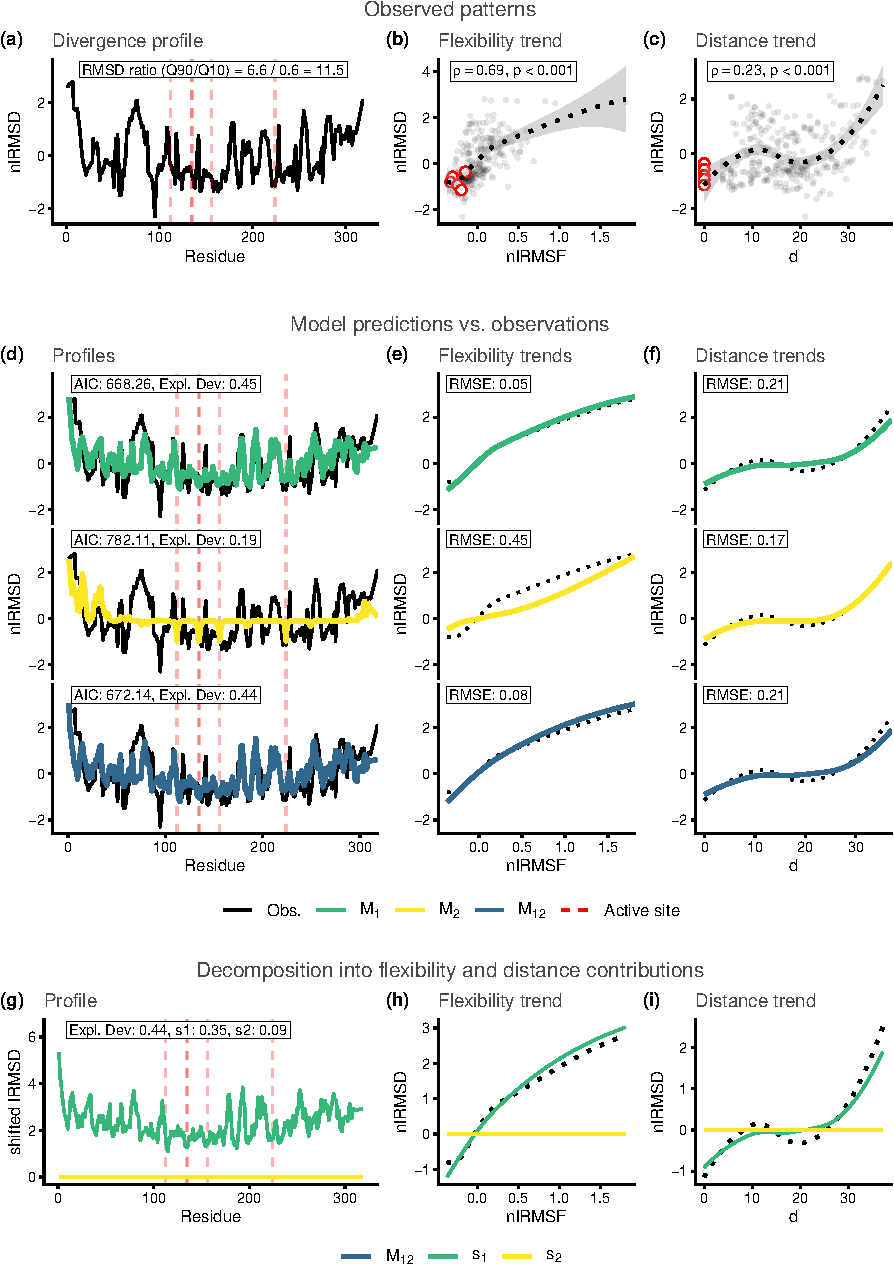
\includegraphics{supplementary_material_files/figure-latex/generate_figures-26} \end{center}

\caption{Structural divergence analysis for enzyme family MCSA ID: 681. Reference protein PDB ID: 1gq8\_A.}
\end{figure}

\clearpage
\begin{figure}[H]
\centering


\begin{center}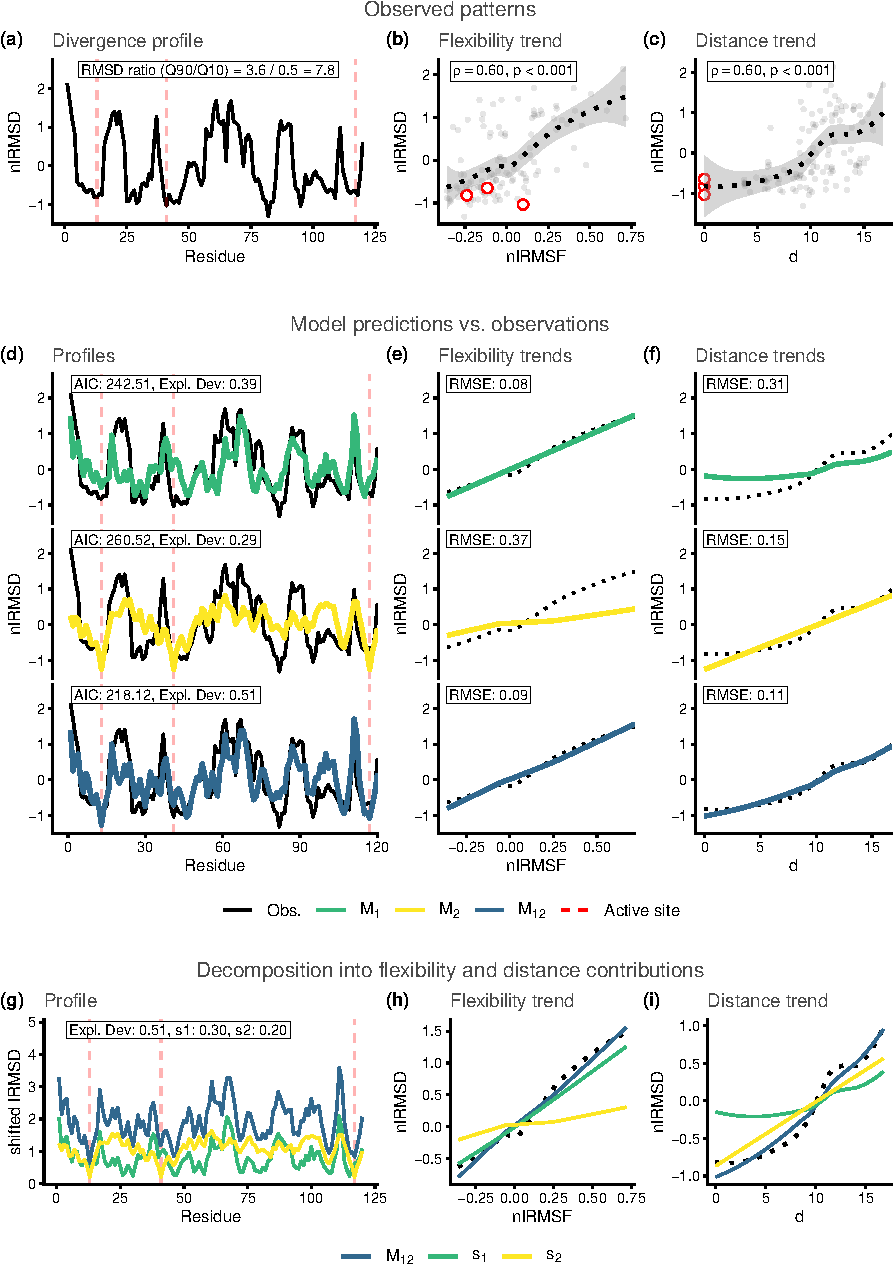
\includegraphics{supplementary_material_files/figure-latex/generate_figures-27} \end{center}

\caption{Structural divergence analysis for enzyme family MCSA ID: 693. Reference protein PDB ID: 2rnf\_A.}
\end{figure}

\clearpage
\begin{figure}[H]
\centering


\begin{center}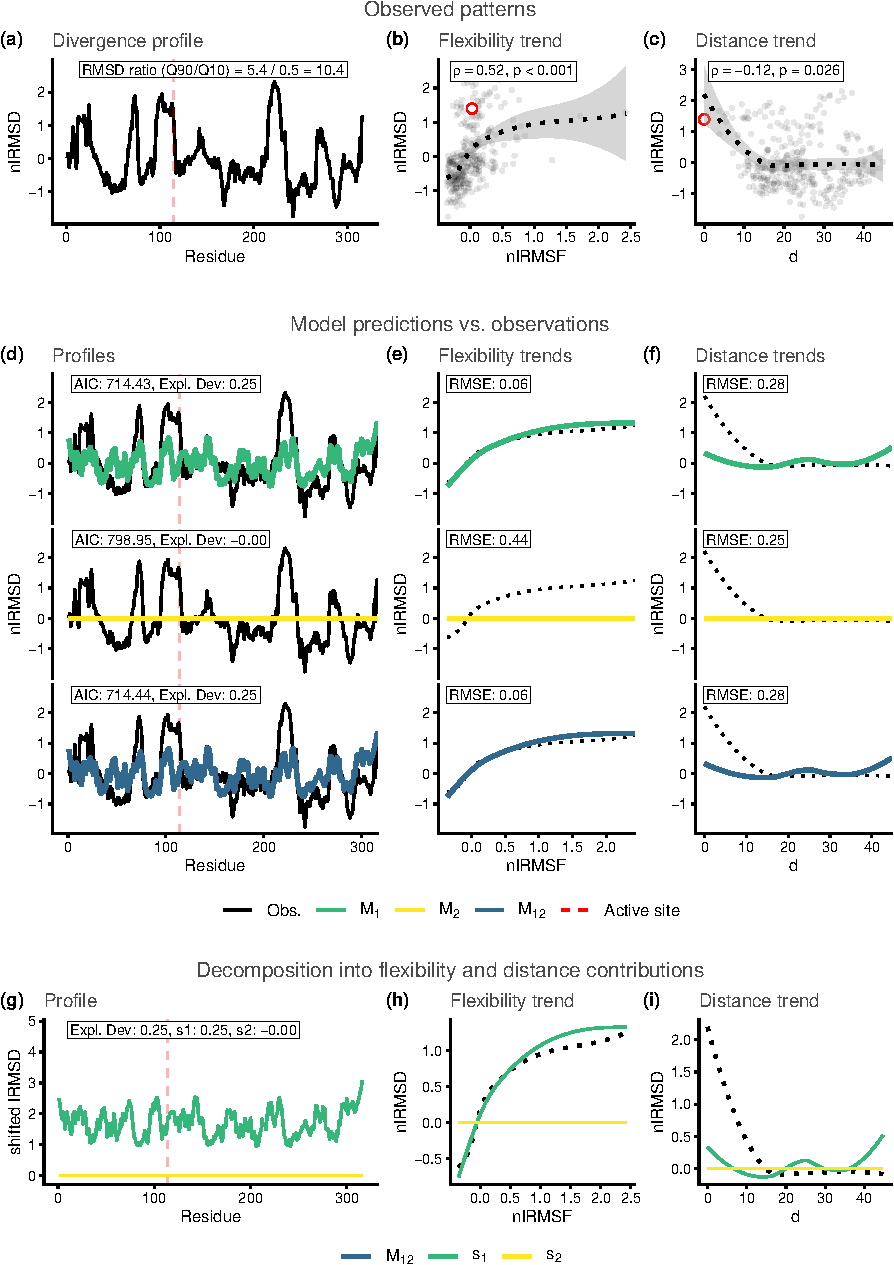
\includegraphics{supplementary_material_files/figure-latex/generate_figures-28} \end{center}

\caption{Structural divergence analysis for enzyme family MCSA ID: 749. Reference protein PDB ID: 1nml\_A.}
\end{figure}

\clearpage
\begin{figure}[H]
\centering


\begin{center}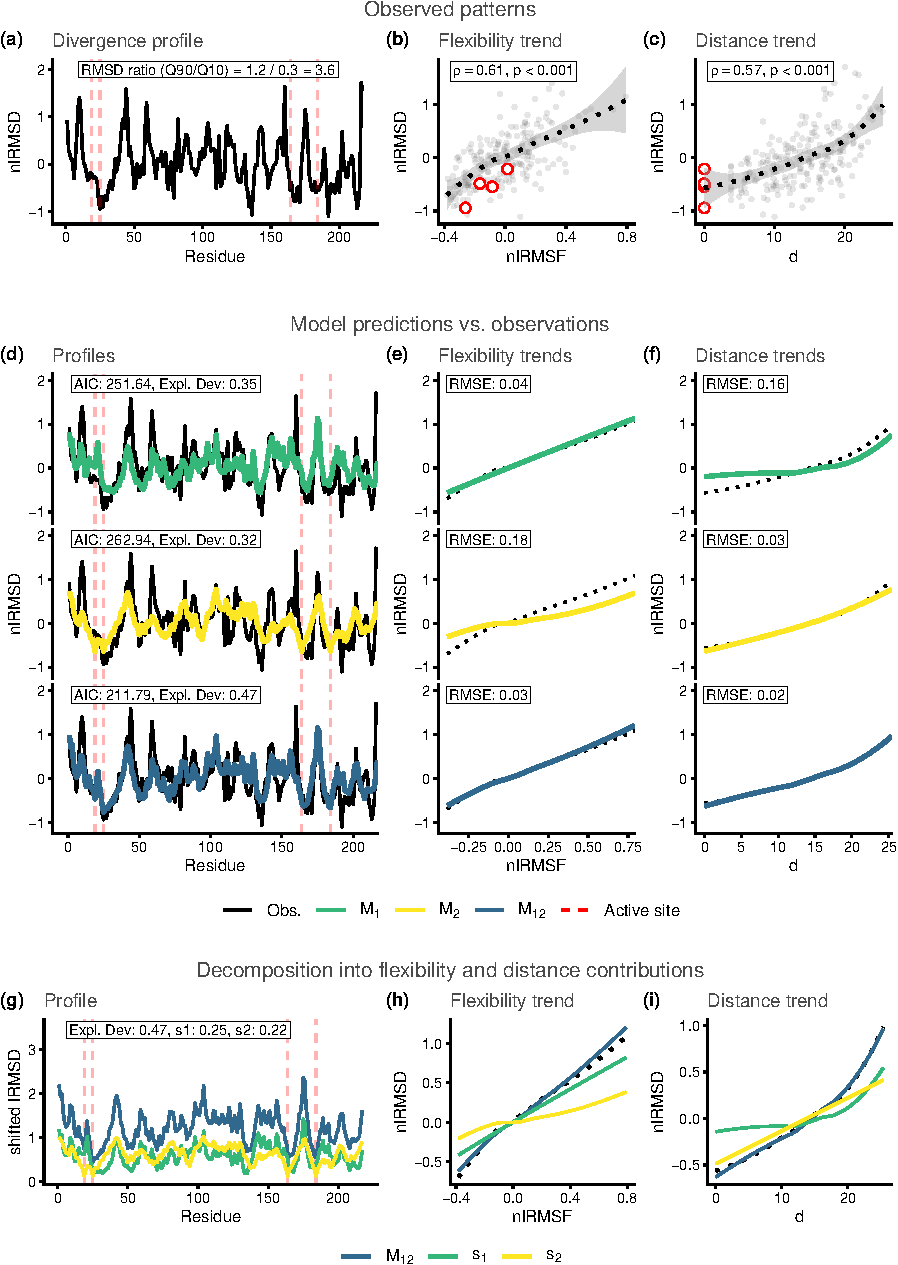
\includegraphics{supplementary_material_files/figure-latex/generate_figures-29} \end{center}

\caption{Structural divergence analysis for enzyme family MCSA ID: 814. Reference protein PDB ID: 1glo\_A.}
\end{figure}

\clearpage
\begin{figure}[H]
\centering


\begin{center}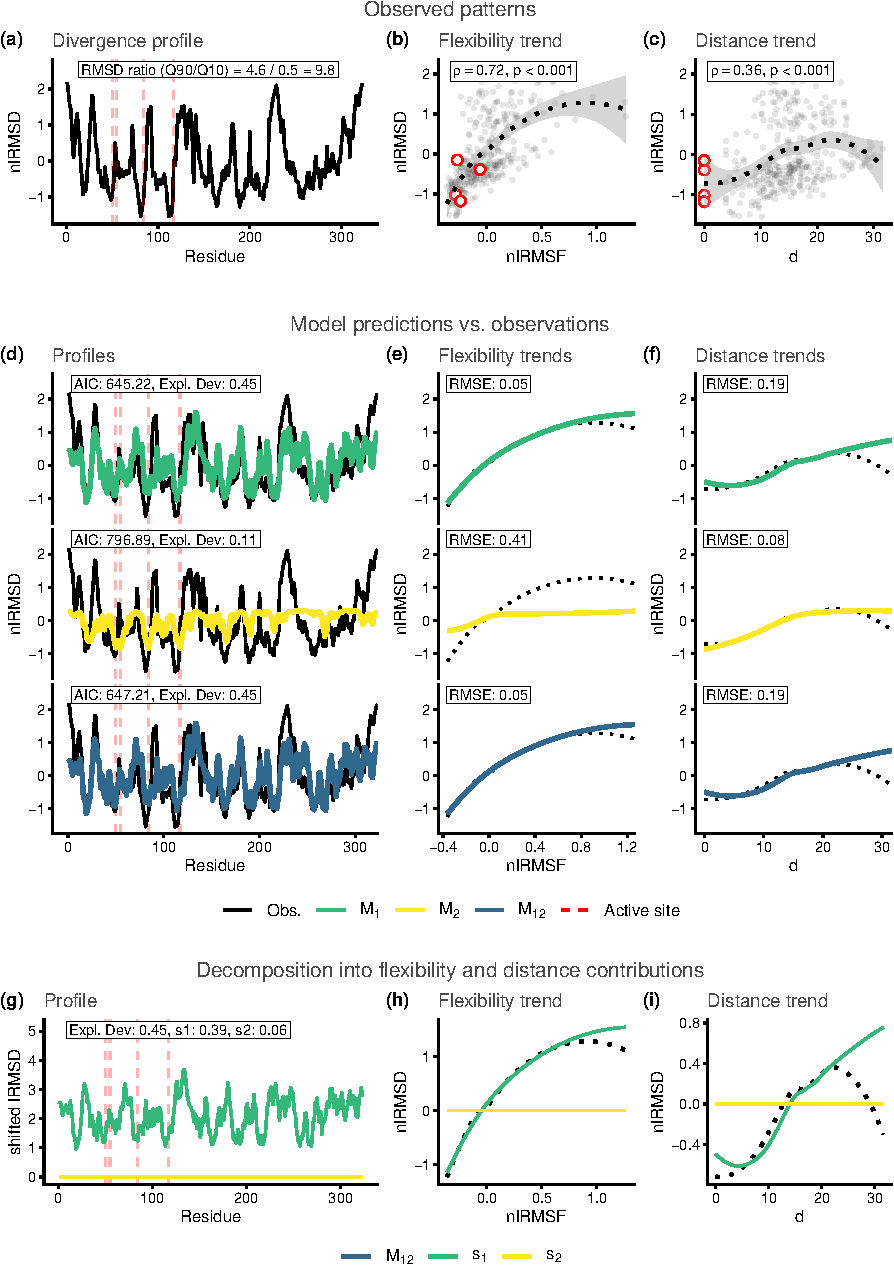
\includegraphics{supplementary_material_files/figure-latex/generate_figures-30} \end{center}

\caption{Structural divergence analysis for enzyme family MCSA ID: 858. Reference protein PDB ID: 1mrq\_A.}
\end{figure}

\clearpage
\begin{figure}[H]
\centering


\begin{center}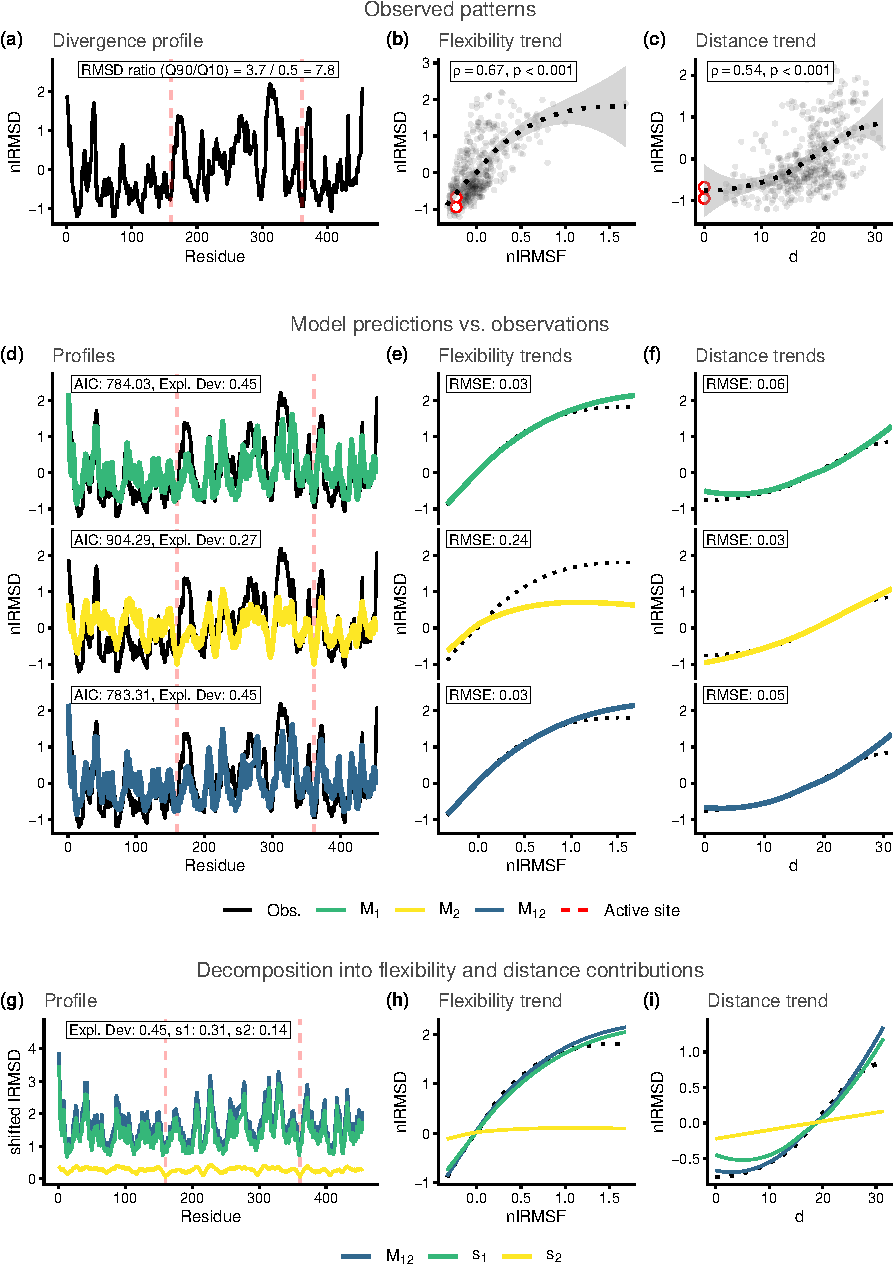
\includegraphics{supplementary_material_files/figure-latex/generate_figures-31} \end{center}

\caption{Structural divergence analysis for enzyme family MCSA ID: 877. Reference protein PDB ID: 1pbg\_A.}
\end{figure}

\clearpage
\begin{figure}[H]
\centering


\begin{center}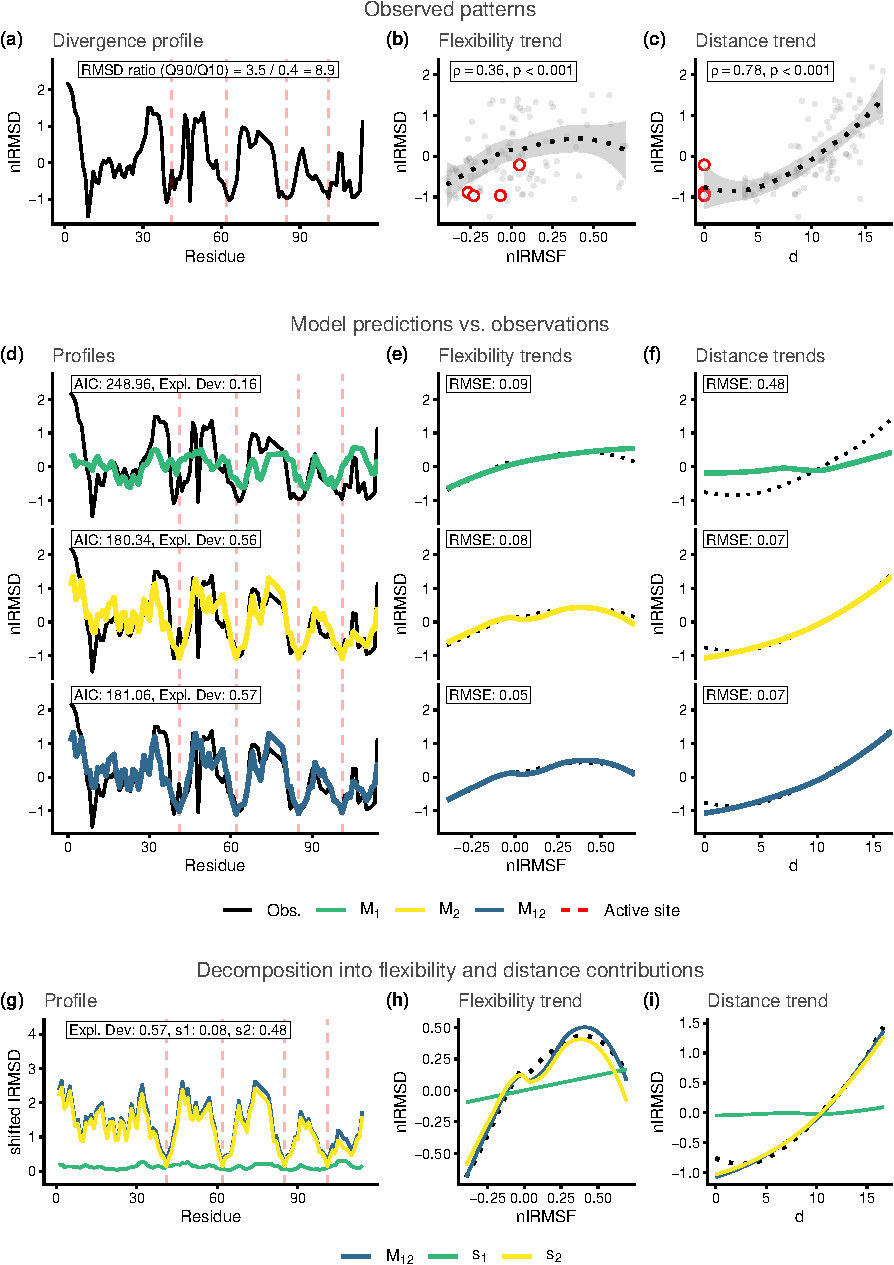
\includegraphics{supplementary_material_files/figure-latex/generate_figures-32} \end{center}

\caption{Structural divergence analysis for enzyme family MCSA ID: 908. Reference protein PDB ID: 1rtu\_A.}
\end{figure}

\clearpage
\begin{figure}[H]
\centering


\begin{center}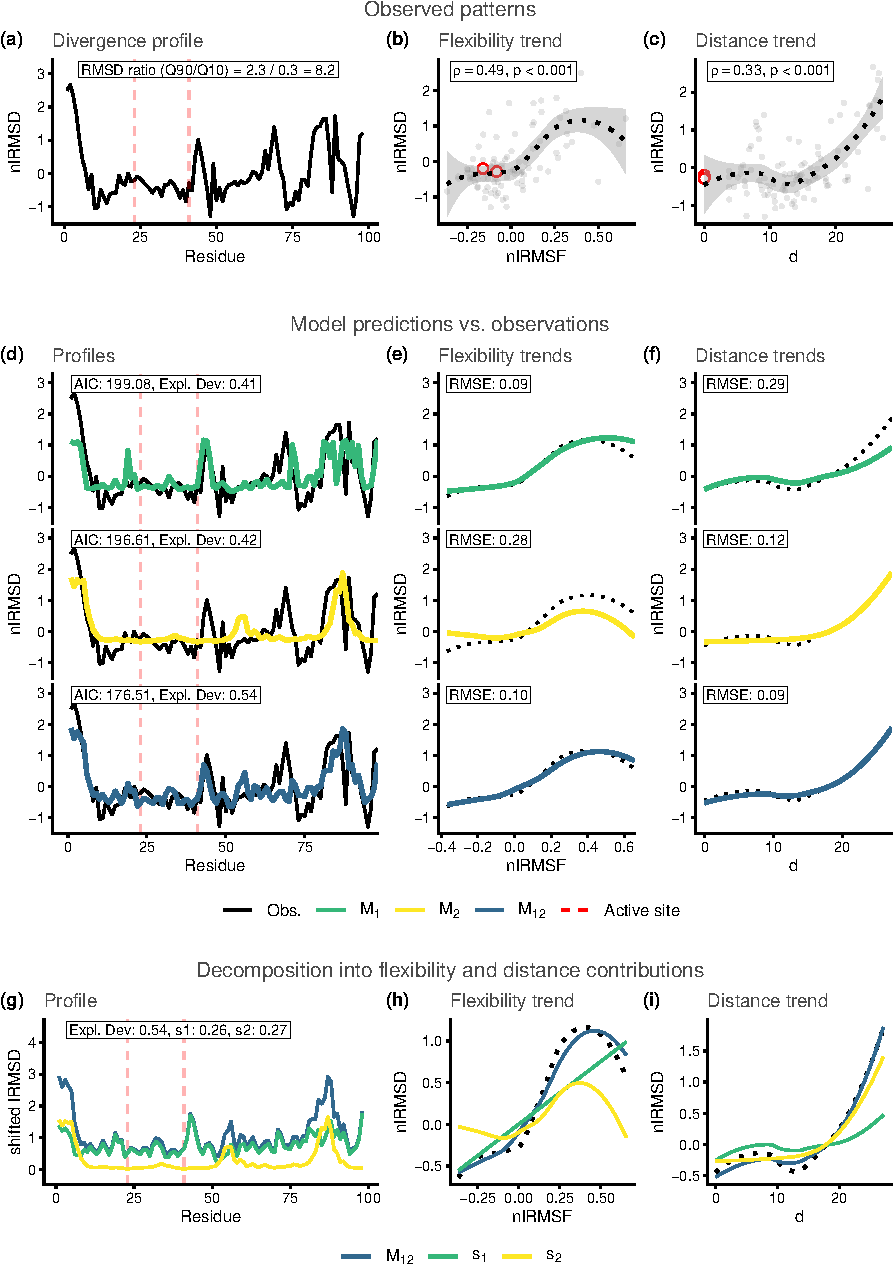
\includegraphics{supplementary_material_files/figure-latex/generate_figures-33} \end{center}

\caption{Structural divergence analysis for enzyme family MCSA ID: 923. Reference protein PDB ID: 2acy\_A.}
\end{figure}

\clearpage
\begin{figure}[H]
\centering


\begin{center}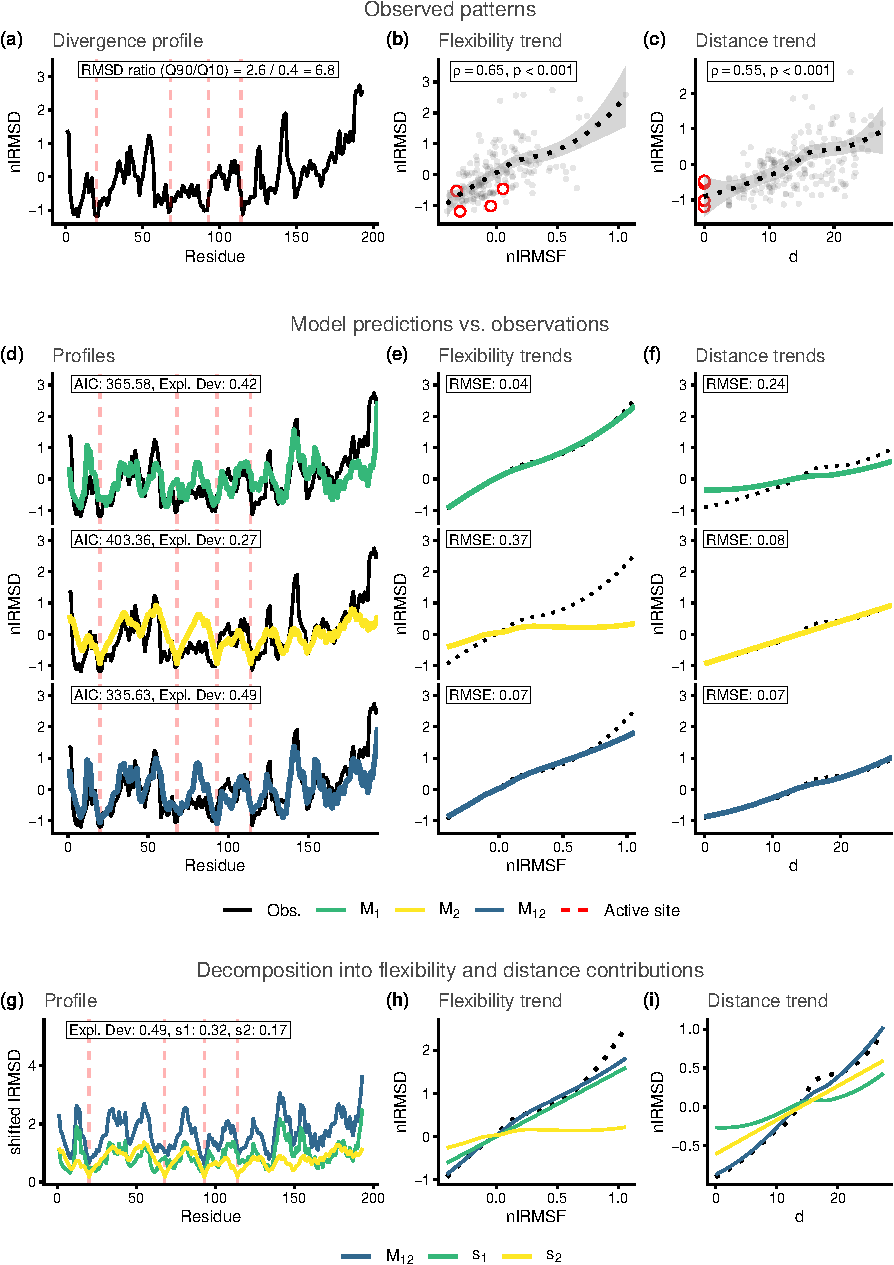
\includegraphics{supplementary_material_files/figure-latex/generate_figures-34} \end{center}

\caption{Structural divergence analysis for enzyme family MCSA ID: 931. Reference protein PDB ID: 2pth\_A.}
\end{figure}

\end{document}
